\documentclass{beamer}

% for themes, etc.
\mode<presentation>
{ \usetheme{metropolis} }
%{ \usetheme{Torino} }
%{ \usetheme{boxes} }

\usepackage{times}  % fonts are up to you
\usepackage{graphicx}
\usepackage{color,colortbl}

\definecolor{MRed}{rgb}{1,.6,.6}
% these will be used later in the title page
\title{ALICE MUON Software for run 3}
\author{Sean Murray \\
    Physics \\
    University of Cape Town 
}
\date{July 6, 2016}

% note: do NOT include a \maketitle line; also note that this title
% material goes BEFORE the \begin{document}

% have this if you'd like a recurring outline
\AtBeginSection[]  % "Beamer, do the following at the start of every section"
{
\begin{frame}<beamer> 
\frametitle{Outline} % make a frame titled "Outline"
\tableofcontents[currentsection]  % show TOC and highlight current section
\end{frame}
}

\begin{document}

% this prints title, author etc. info from above
\begin{frame}
\titlepage
\end{frame}

\section{ALICE}

\begin{frame}
\frametitle{ALICE}

  \center{
  
\includegraphics[scale=0.35,trim={5cm 2cm 3cm 4cm},clip]{images/pg_0004.pdf}
  }
\end{frame}


\section{O2 and Run3}
\begin{frame}
\frametitle{O2 Online/Offline}
We will not go into depth, this is a whole other presentation.
Important numbers to take away :
\begin{itemize}
  \item 50kHz event rate.
  \item 1.1 TB/s aggregate data rate.
  \item continuous read out for most detectors, TPC and MUON joint chip design.
  \item Completely new framework.
  \item merge HLT, data acquisition and offline into 1 code base and platform.
  \item calibration and reconstruction online.
  \item Collaboration with FAIR for new framework.
\end{itemize}

\end{frame}
\begin{frame}
  \frametitle{O2 Farm}
  \center{
  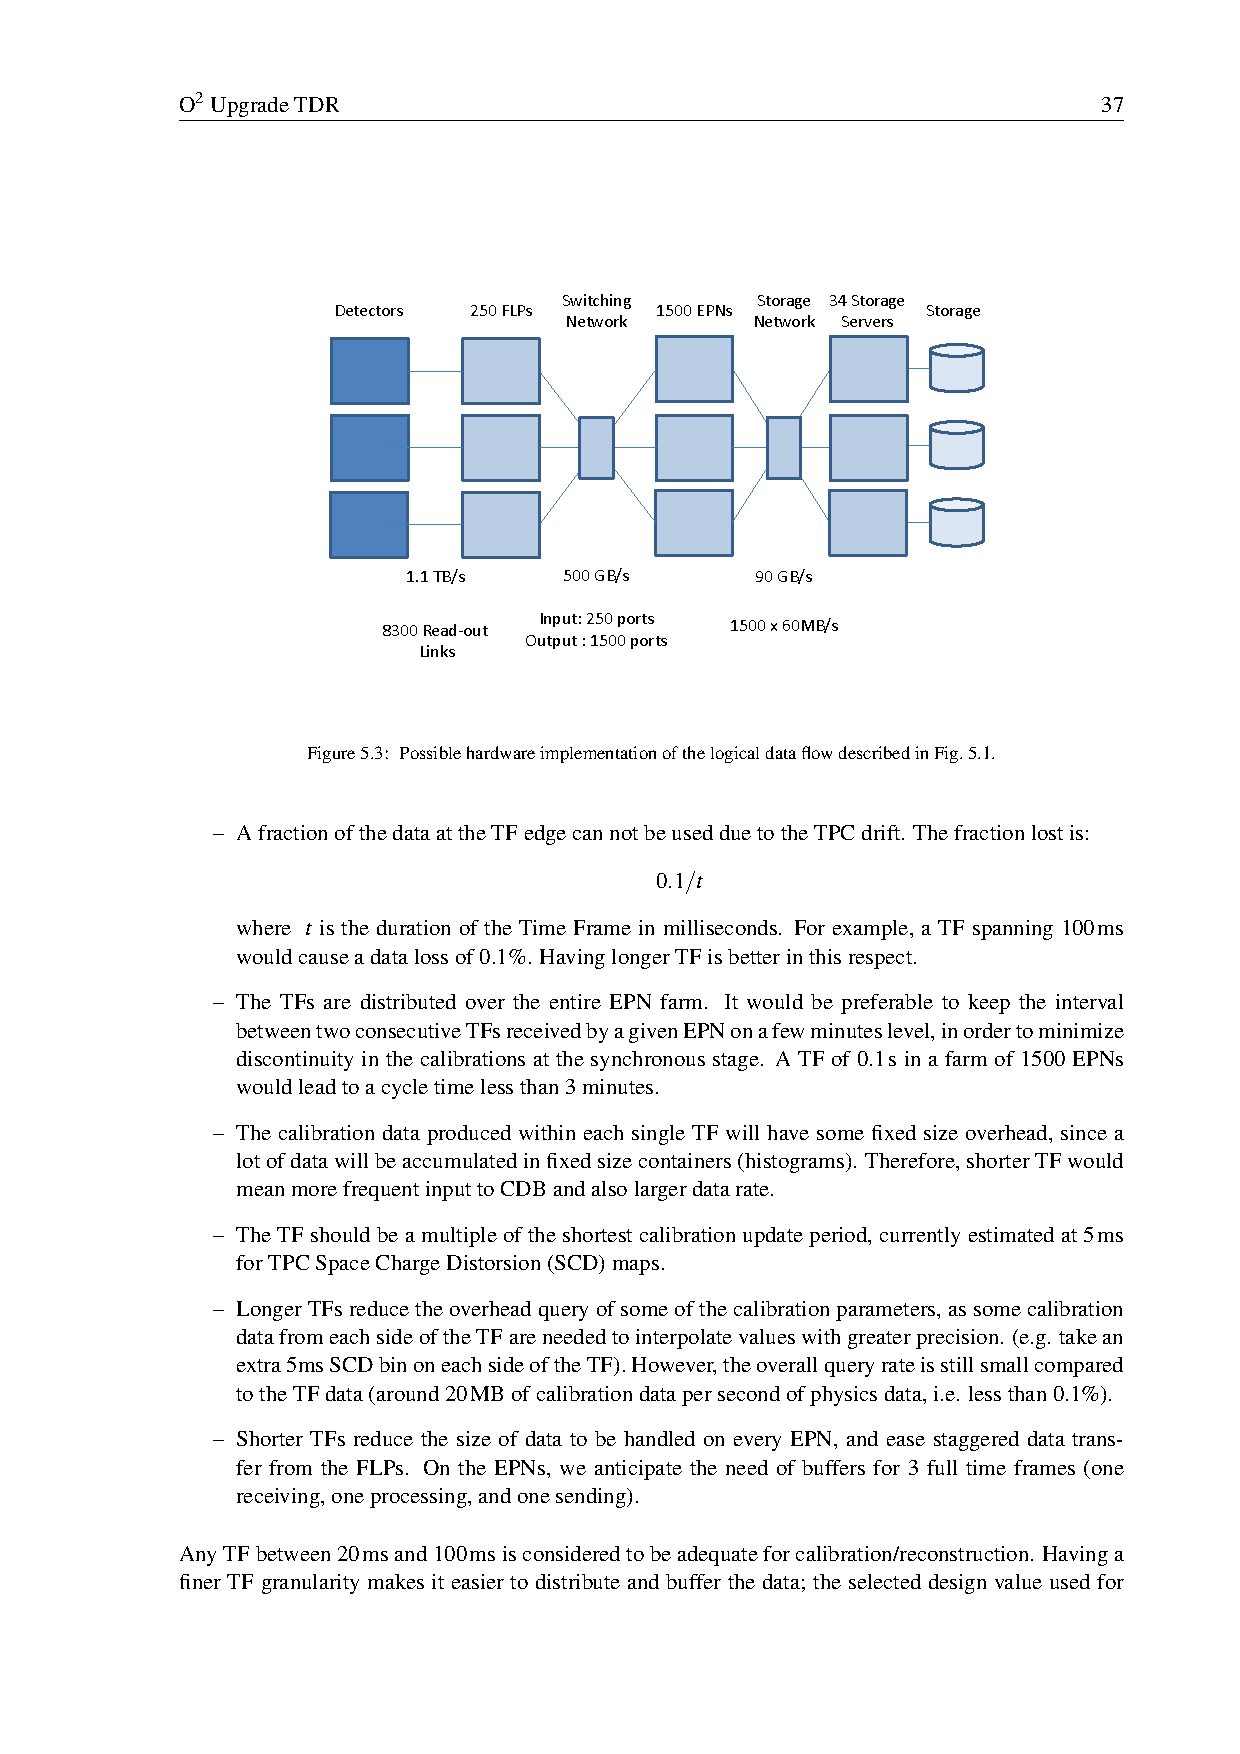
\includegraphics[scale=0.7,trim={3cm 18cm 3cm 3cm},clip]{images/ALICE_TDR-019_49.pdf}
  }
\end{frame}

\begin{frame}
  \frametitle{MUON Links}
  \tiny{\begin{tabular}{|l|l|r|r|r|l|r|r|}
   Detector  &      Link    &  \multicolumn{3}{c}{ Number of links}   &     Read-out &   \multicolumn{2}{c}{Number of boards} \\
             &      type    & DDL1& DDL2 &  GBT  &  board type&   C-RORC& CRU \\ \hline\hline
    ACO      &     DDL1     &  1  &      &       &  C-RORC    &      1   &   \\ 
    CPV      &     DDL1     &  6  &      &       &  C-RORC    &      1   &\\ 
    CTP      &    GBT       &     &      &    14 &  CRU       &          &     1\\ 
    EMC      &   DDL2       &     &   20 &       &  C-RORC    &      4   &\\ 
    FIT      &     DDL2     &     &    2 &       &  C-RORC    &      1   &\\ 
    HMP      &     DDL1     &  14 &      &       &  C-RORC    &      4   &\\ 
    ITS      &     GBT      &     &      &   495 &  CRU       &          &               23\\ 
\rowcolor{MRed}    MCH      &     GBT      &     &      &   550 &  CRU       &          &               25\\ 
\rowcolor{MRed}    MFT      &     GBT      &     &      &   304 &  CRU       &          &               14\\ 
\rowcolor{MRed}    MID      &     GBT      &     &      &    32 &  CRU       &          &                2\\ 
    PHS      &     DDL2     &     &      &    16 &  C-RORC    &     4    &\\ 
    TOF      &     GBT      &     &      &    72 &  CRU       &          &               3\\ 
    TPC      &     GBT      &     &      &  5832 &  CRU       &          &             324\\ 
    TRD      &     Custom   &     &      &  1044 &  CRU       &          &              54\\ 
    ZDC      &     GBT      &     &      &     1 &  CRU       &          &               1\\  \hline
    Total    &               & 21 &  38  &  8344 &            &   15     &          447\\ 
            \end{tabular}}\\
            \vspace{1cm}
            Muon therefore get 6 FLPs
\end{frame}


\section{ALICE Muons}

\begin{frame}
\frametitle{ALICE MUON Arm}
  \center{
  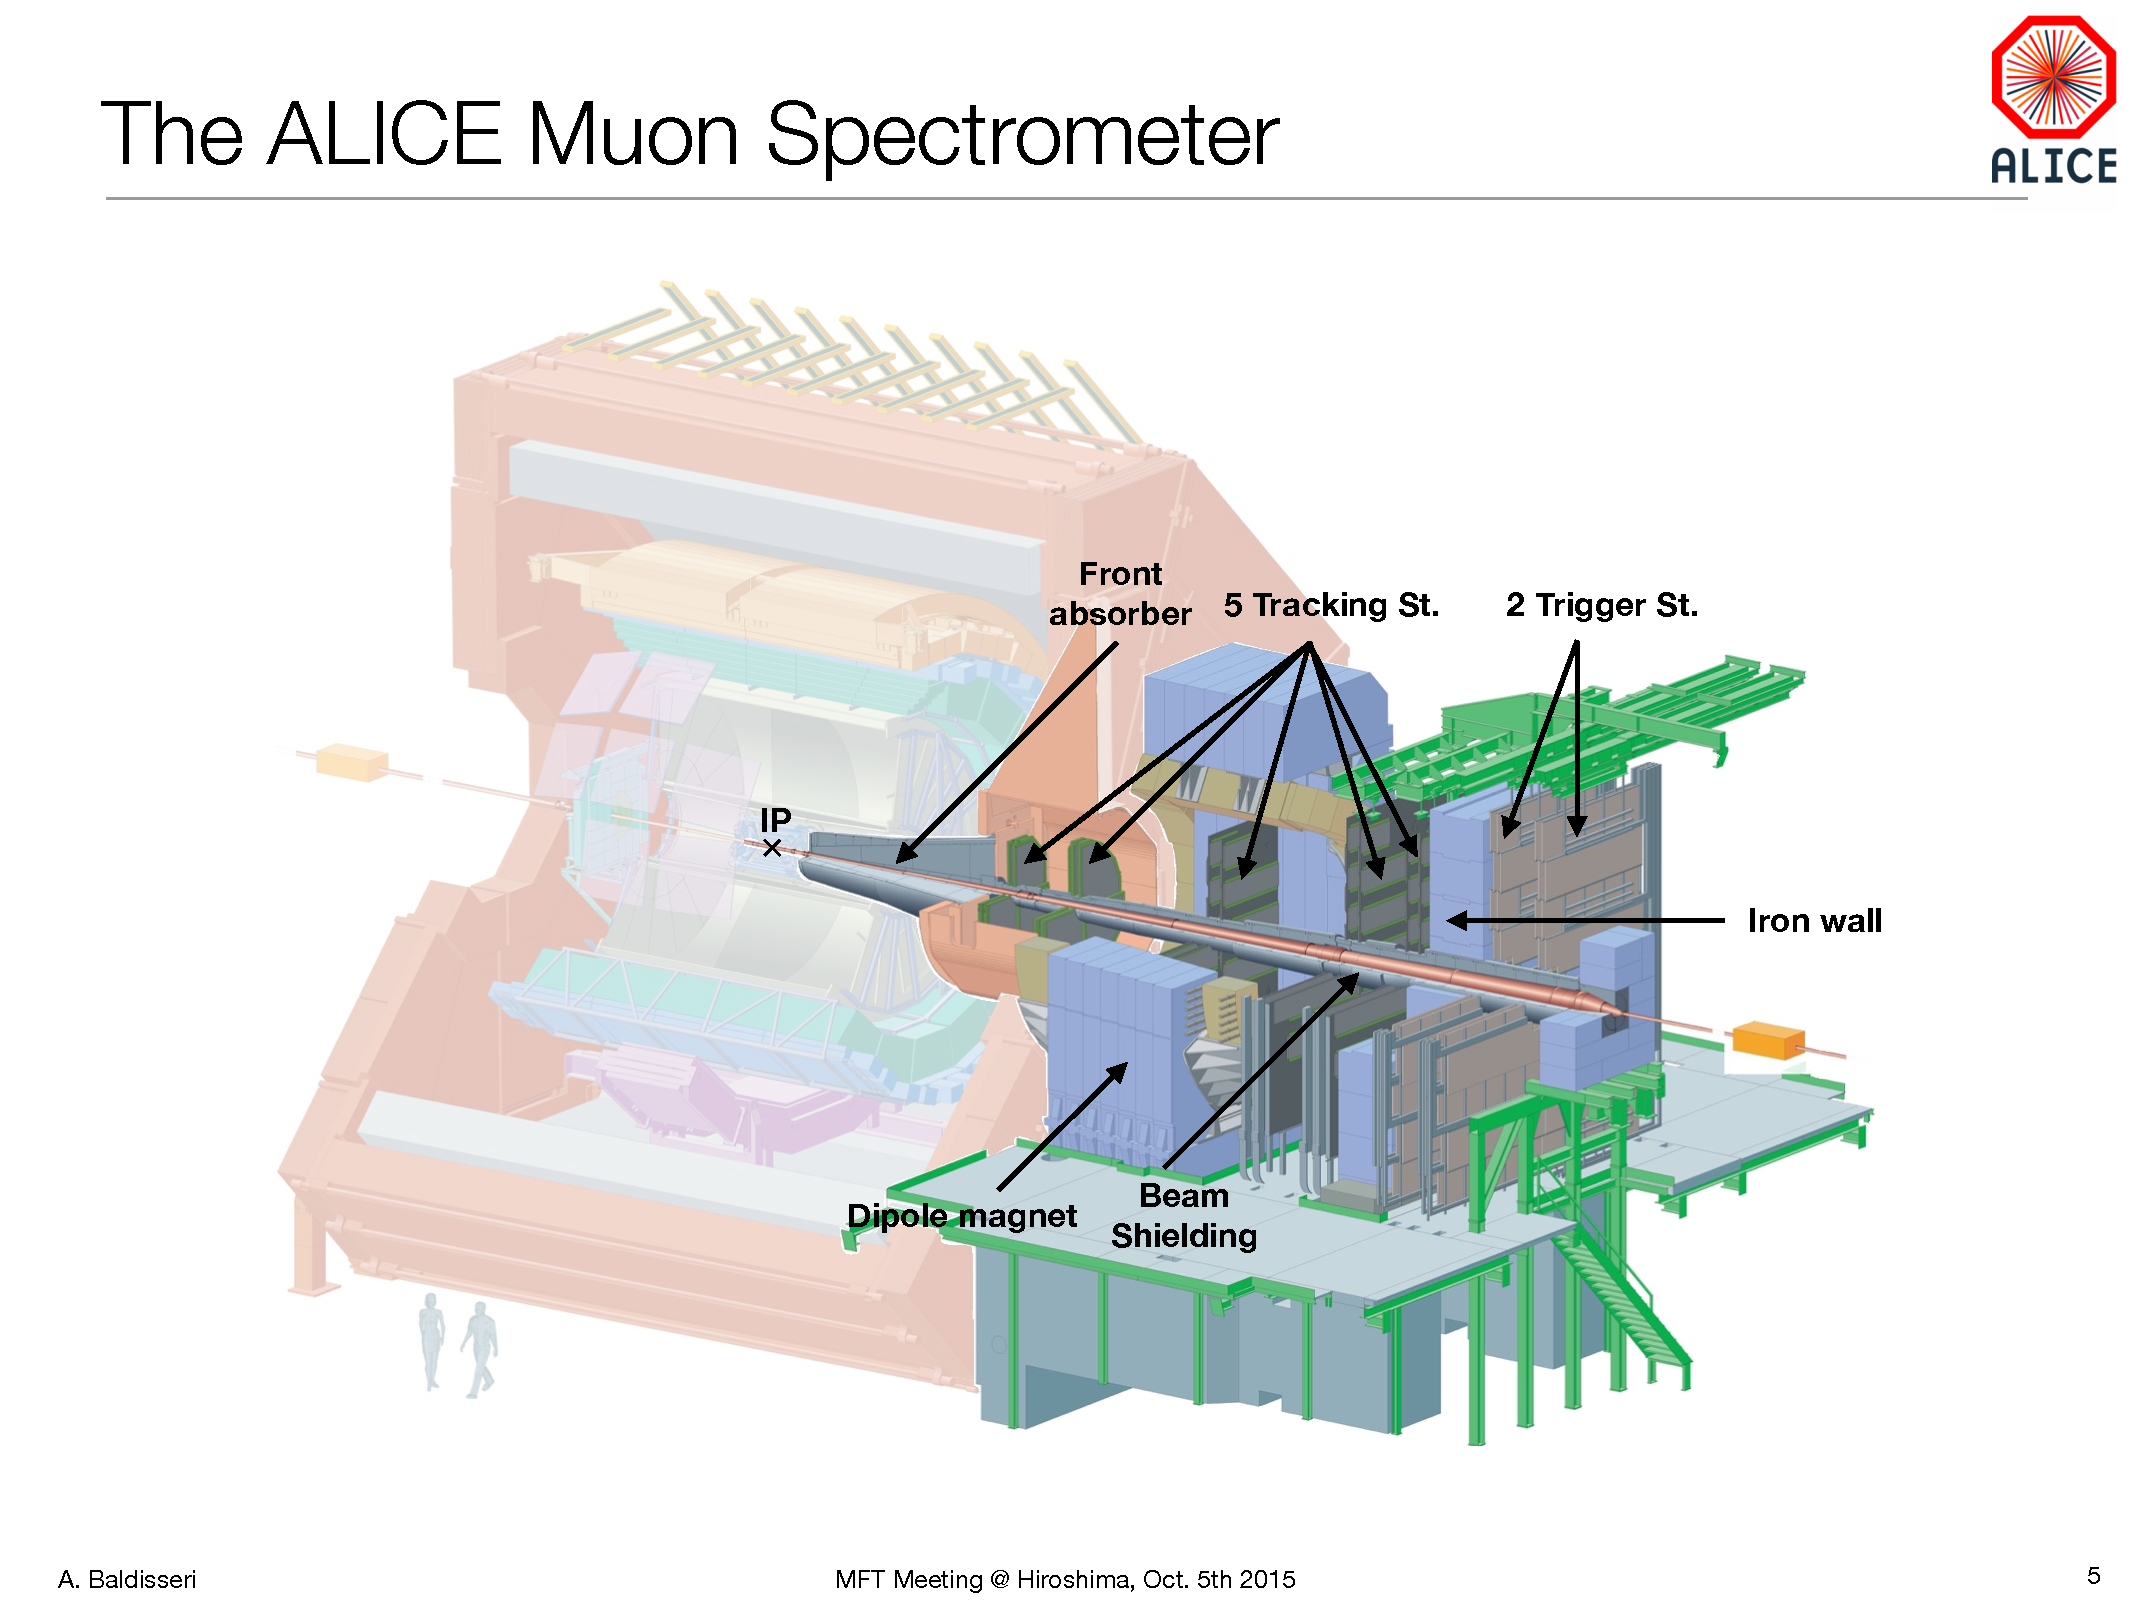
\includegraphics[scale=0.35,trim={3cm 1cm 3cm 4cm},clip]{images/pg_0005.pdf}
  }
\end{frame}
\begin{frame}
  \frametitle{ALICE MUON diagram}

  \center{
  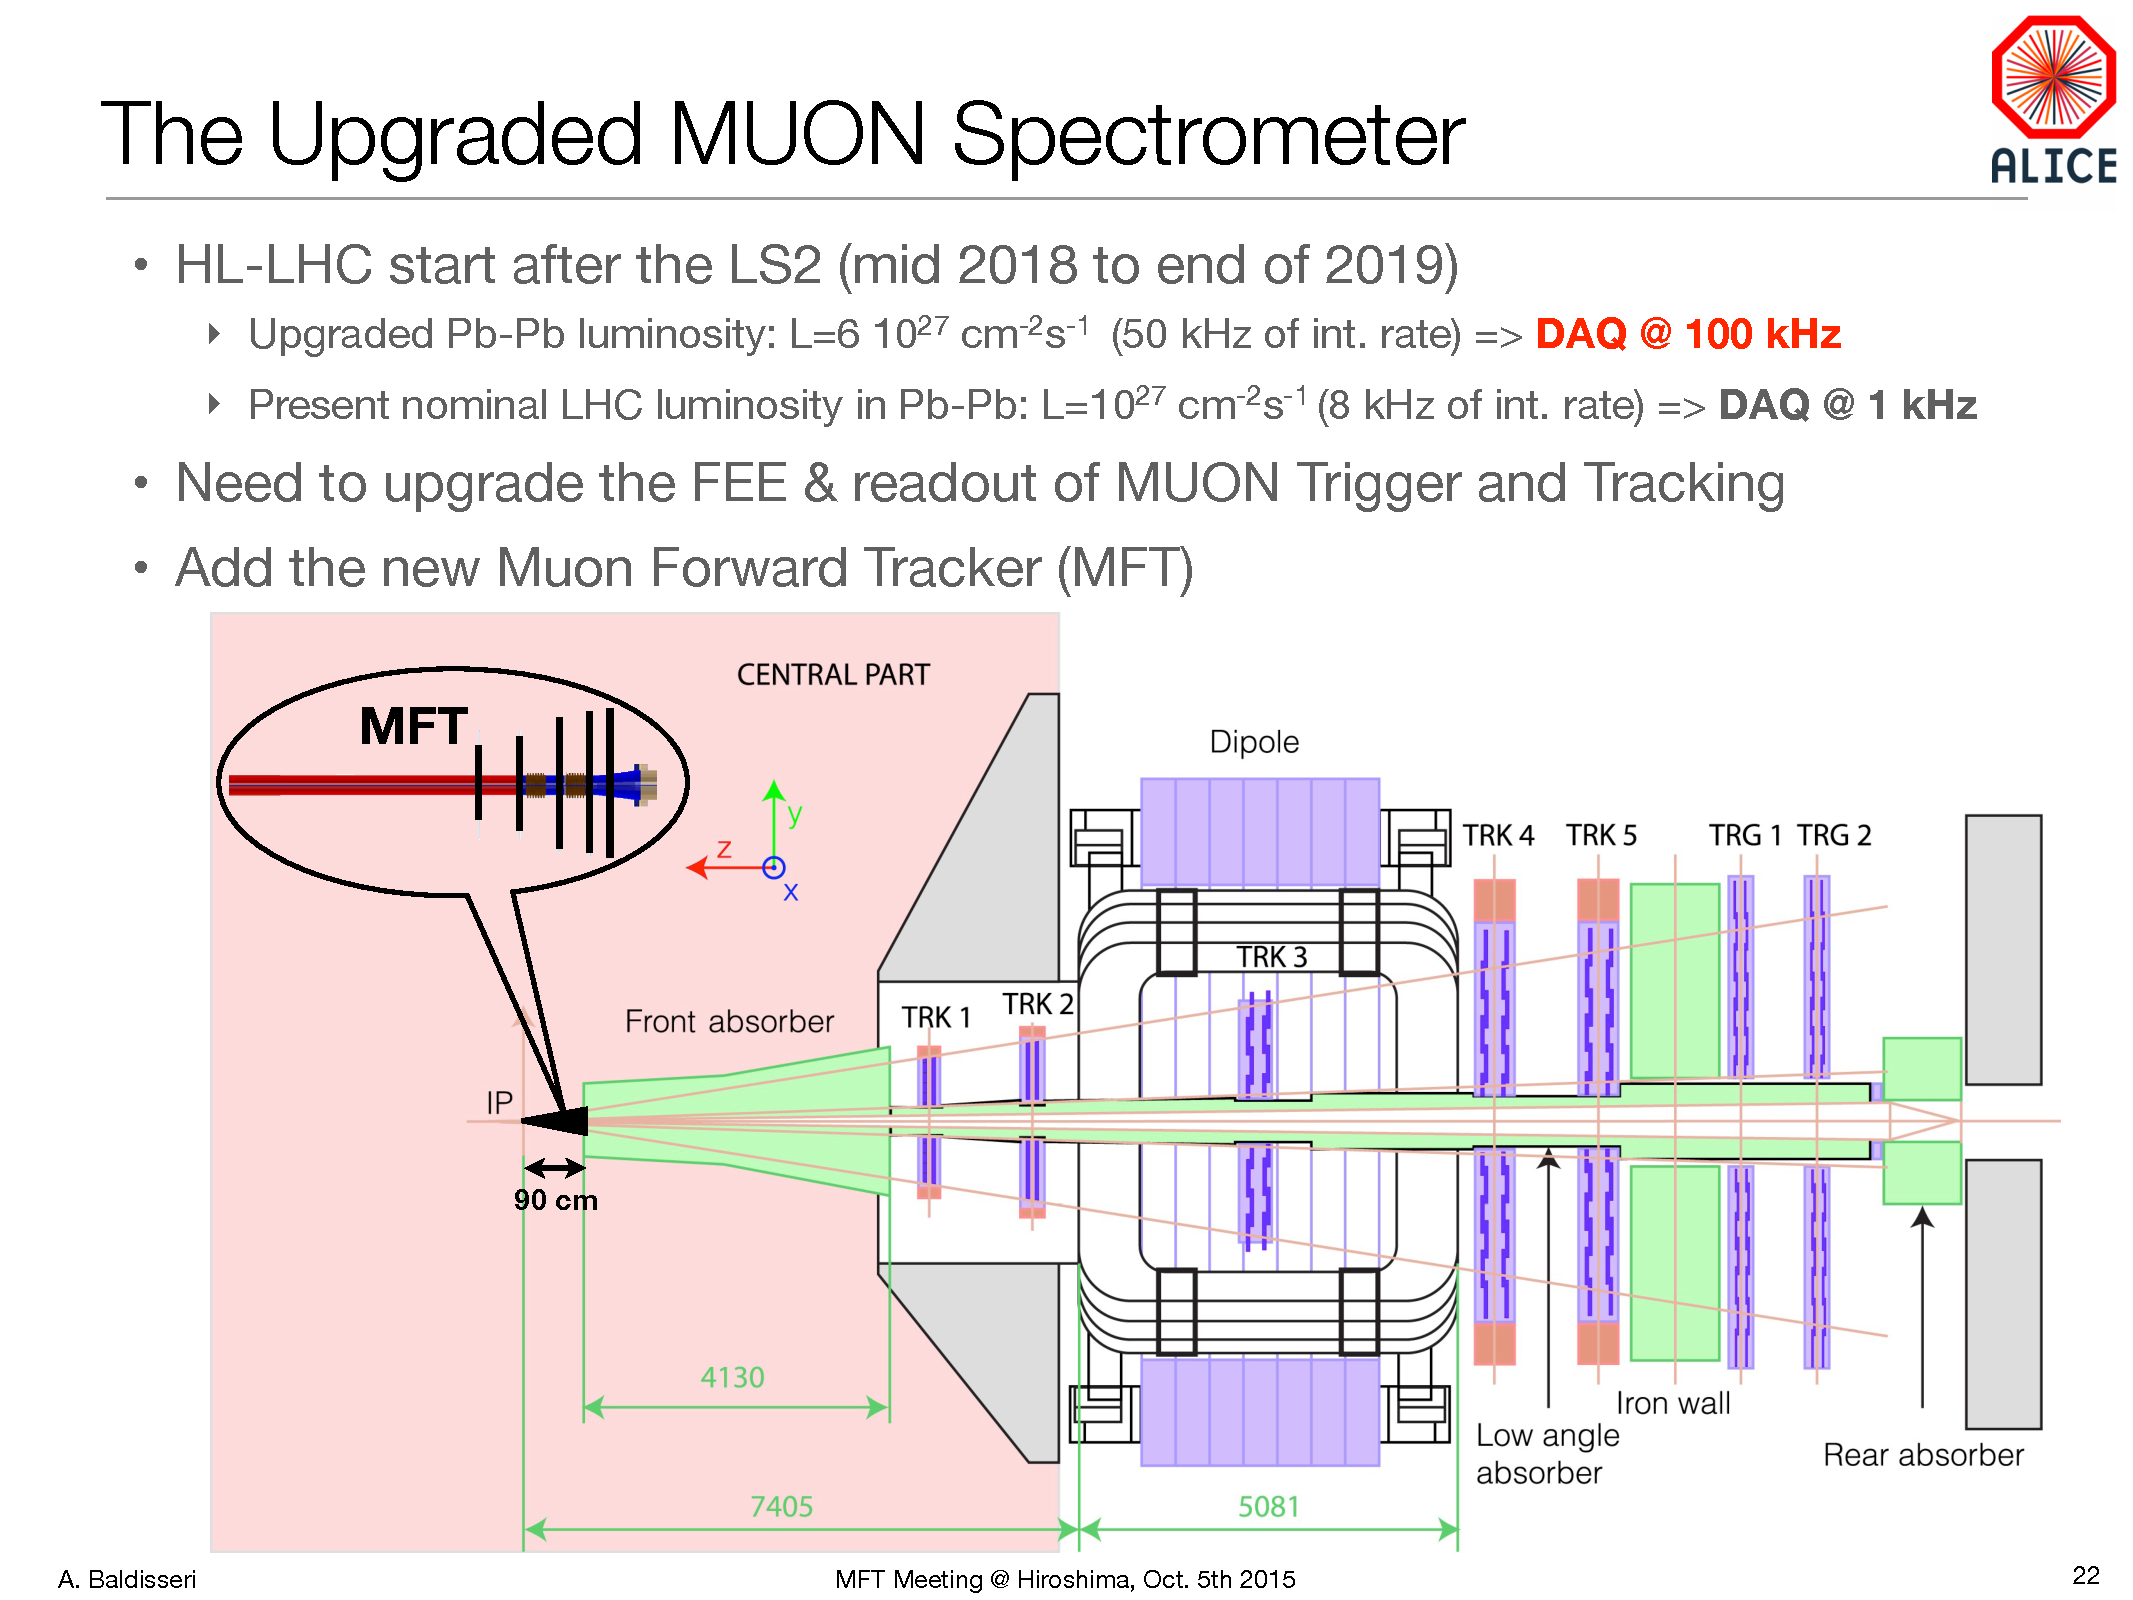
\includegraphics[scale=0.35,trim={2cm 0.75cm 1cm 10cm},clip]{images/pg_0022.pdf}
  }

\end{frame}

\begin{frame}
\frametitle{Detector Structure Station1}
\centering{
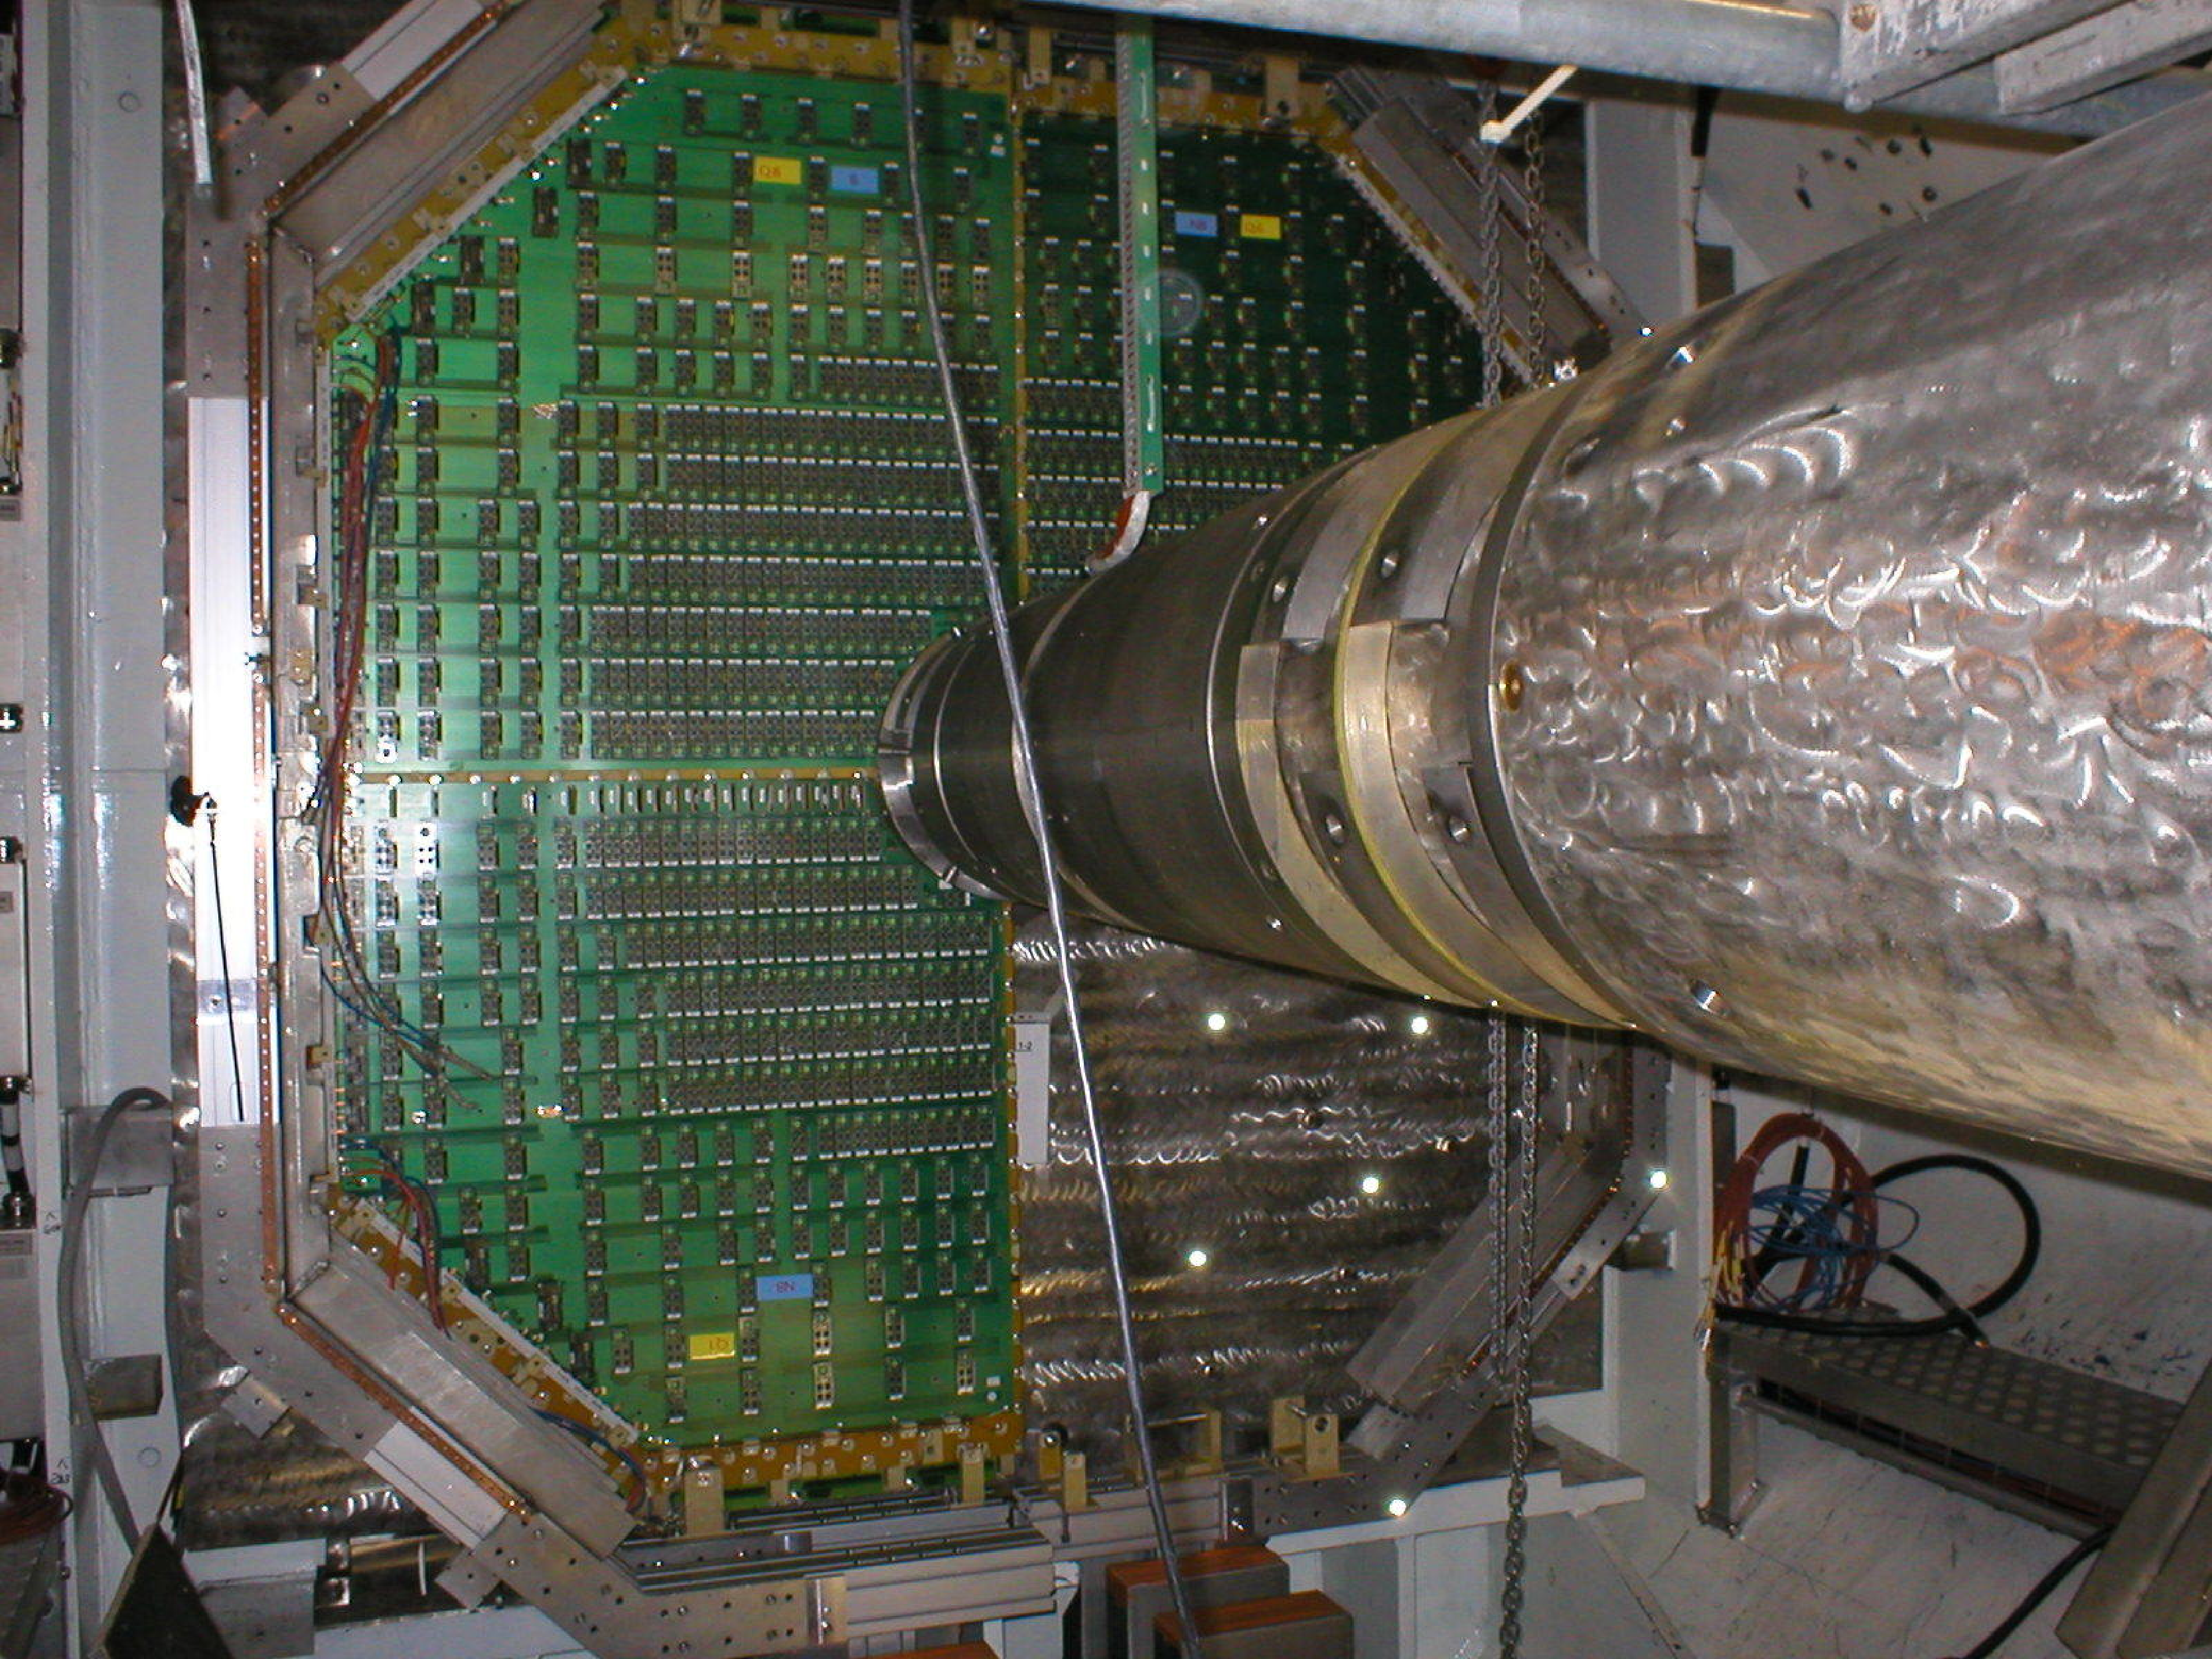
\includegraphics[scale=0.25]{images/MuonStation1.pdf}
} 
\end{frame}


\begin{frame}
\frametitle{Detector Structure Station1 quadrant}
\centering{
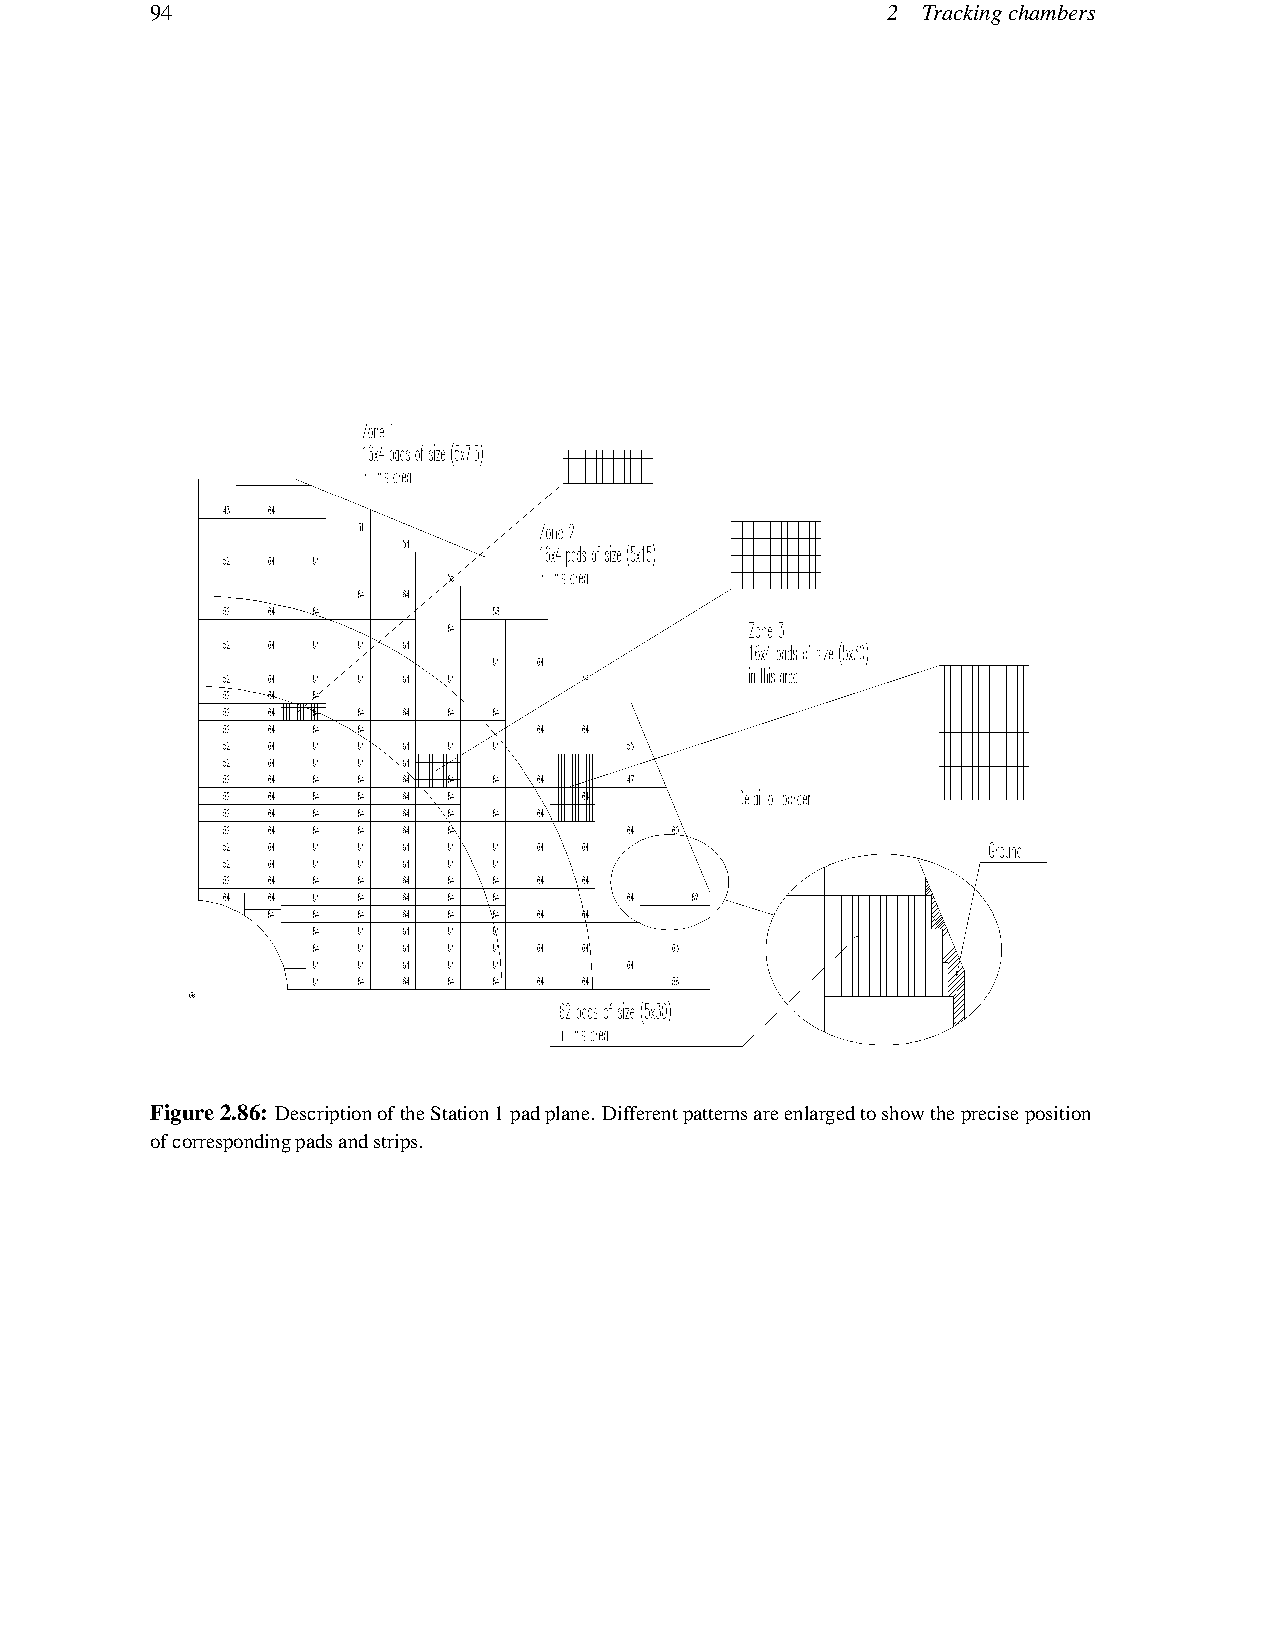
\includegraphics[scale=0.75,trim={2cm 7cm 3cm 7cm},clip]{images/Station1Wires.pdf}
} \\
\end{frame}

\begin{frame}
\frametitle{Detector Slats}
\centering{
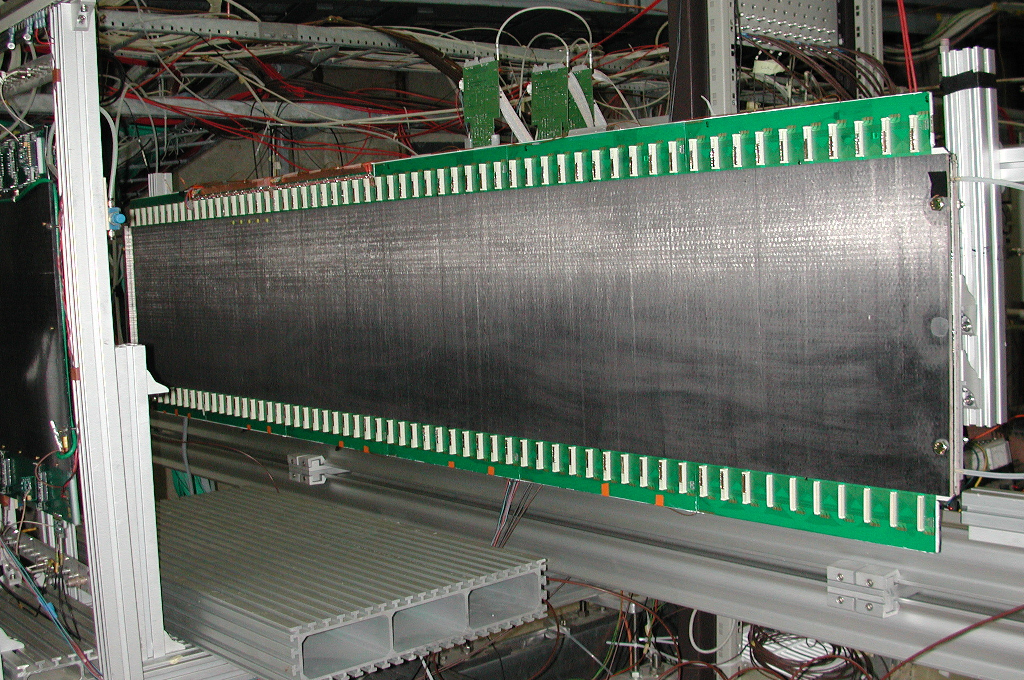
\includegraphics[scale=0.5]{images/MUONSlat.pdf}
} 
\end{frame}
%\begin{frame}
%\frametitle{Detector Slats in place}
%\centering{
%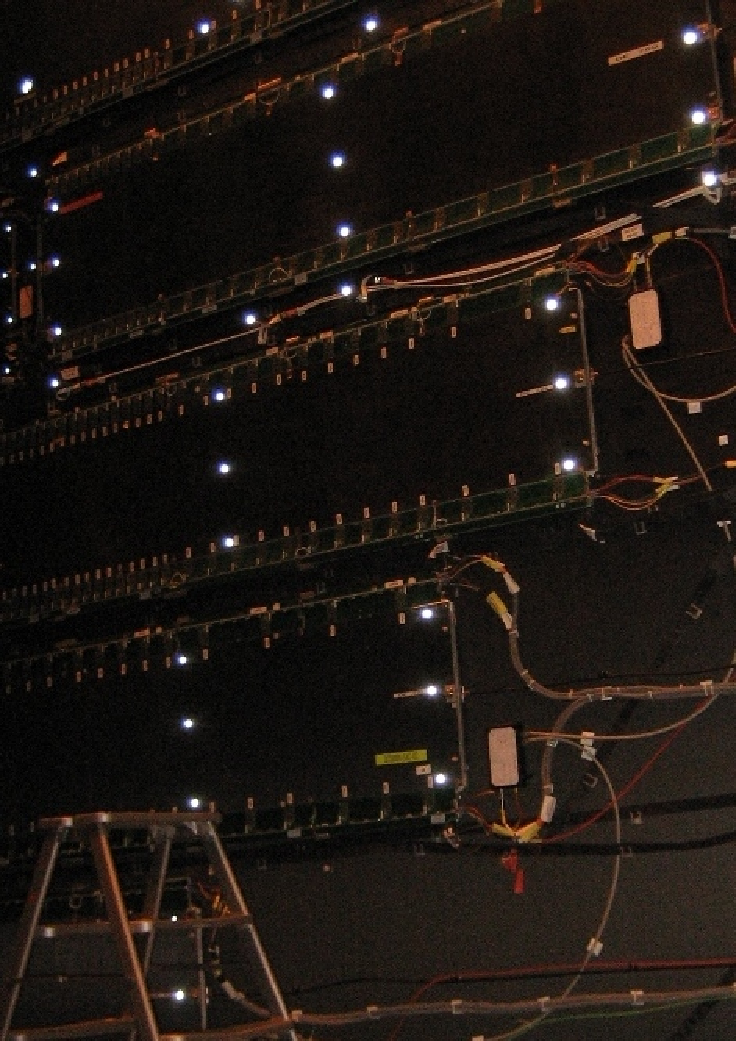
\includegraphics[scale=0.5]{images/MUONSlatsIn.pdf}
%} 
%\end{frame}


\begin{frame}
\frametitle{MUON Slats through the Dipole}
\centering{
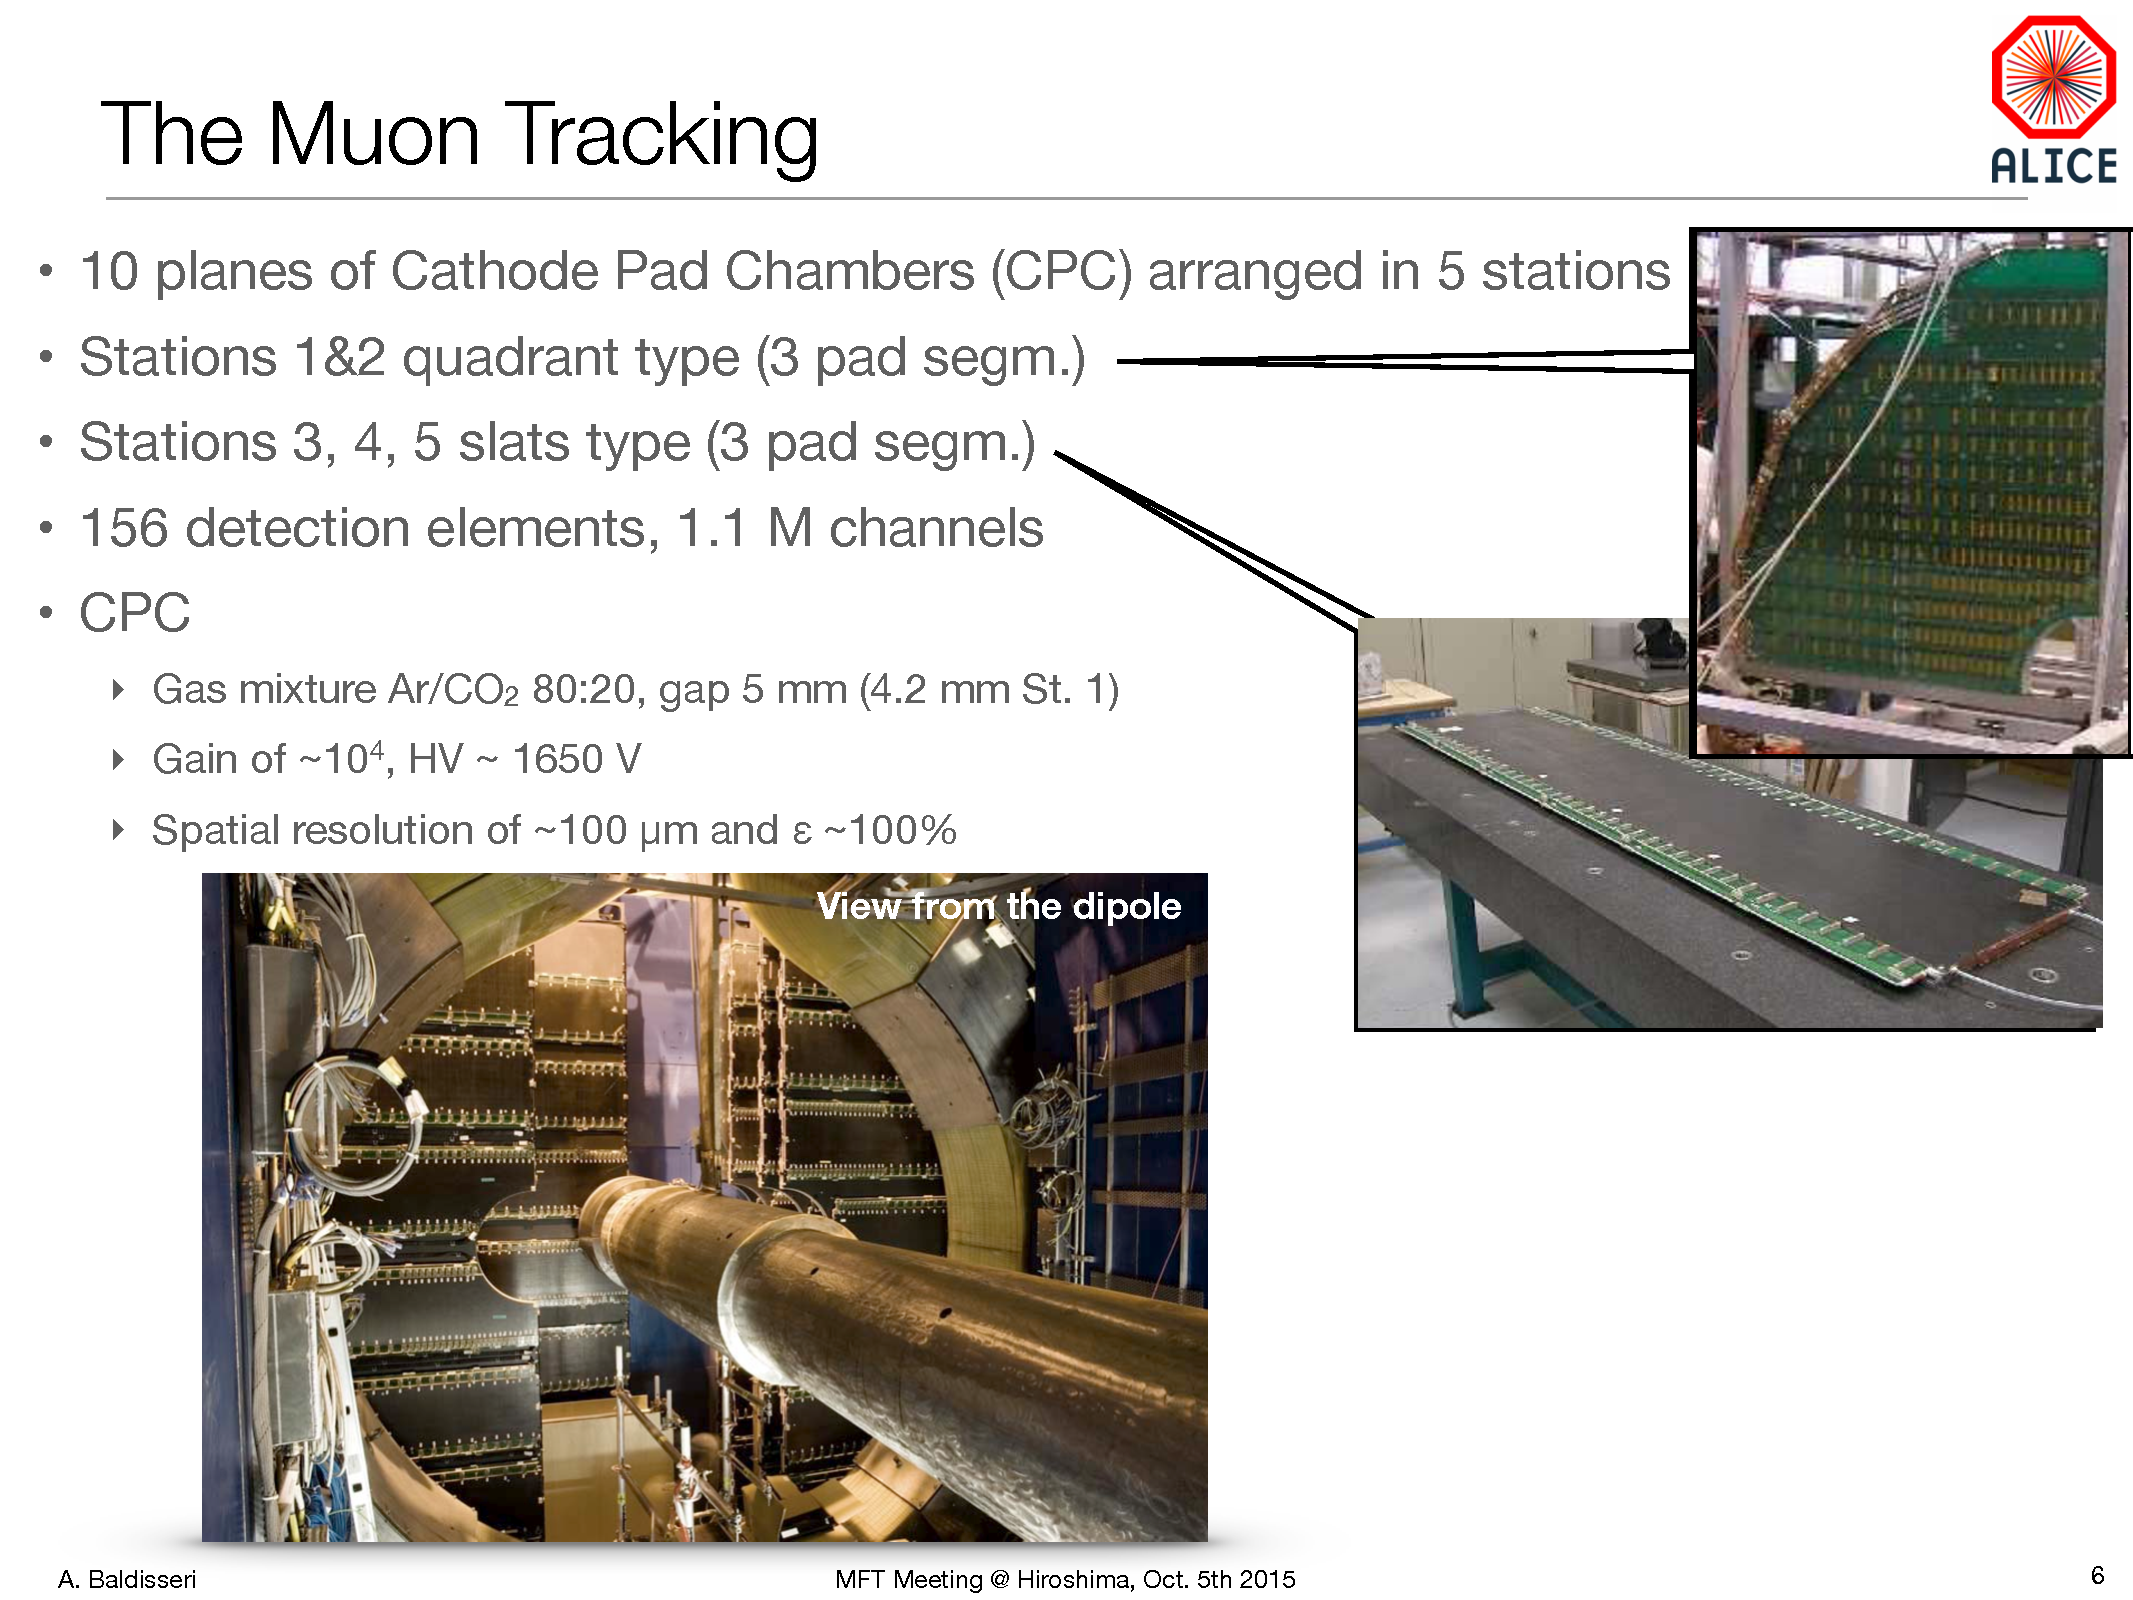
\includegraphics[scale=0.5, trim={2cm 1cm 17cm 16cm},clip]{images/pg_0006.pdf}
} \\

\end{frame}

\begin{frame}
\frametitle{Detector Slats schematic}
\centering{
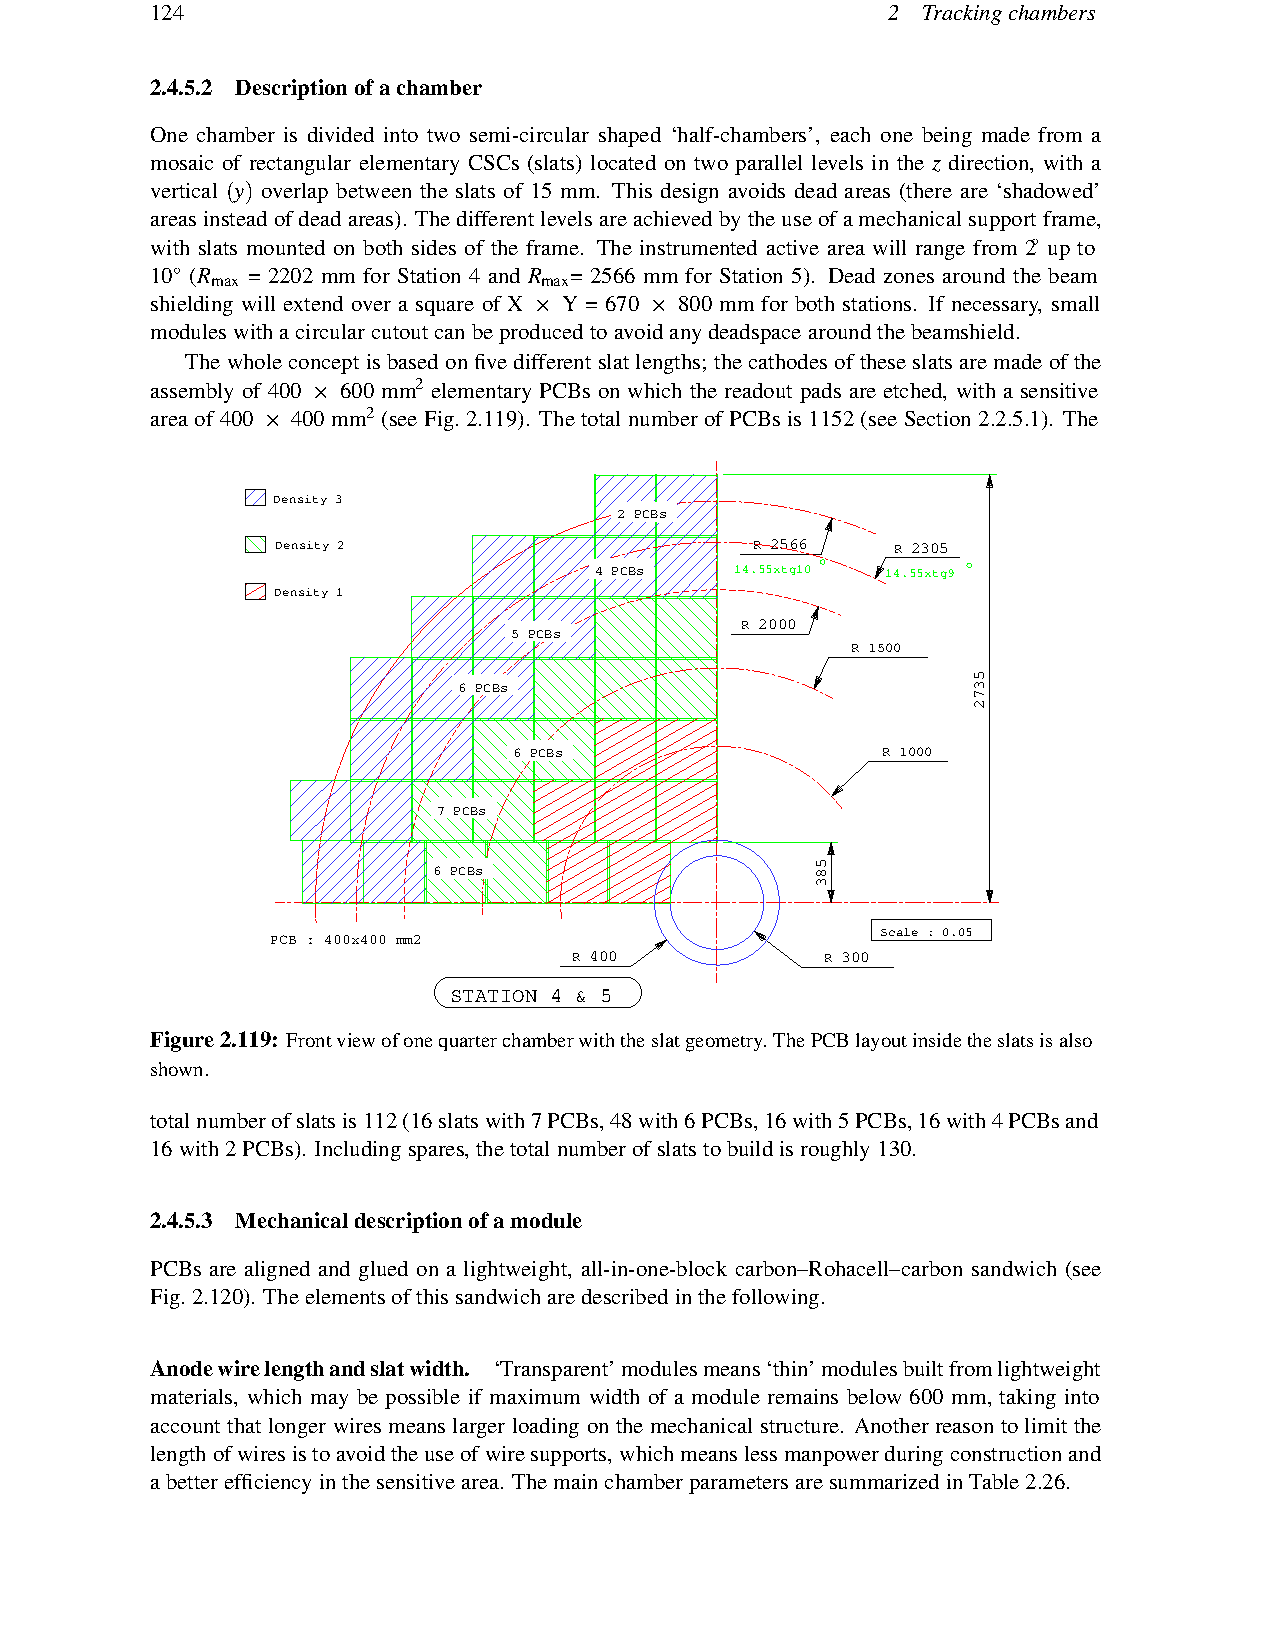
\includegraphics[scale=0.75, trim={4cm 10.5cm 2cm 8cm},clip]{images/Chapter2-2_pages_24.pdf}
} 
\end{frame}


\begin{frame}
  \frametitle{Nominal pp event}
\centering{
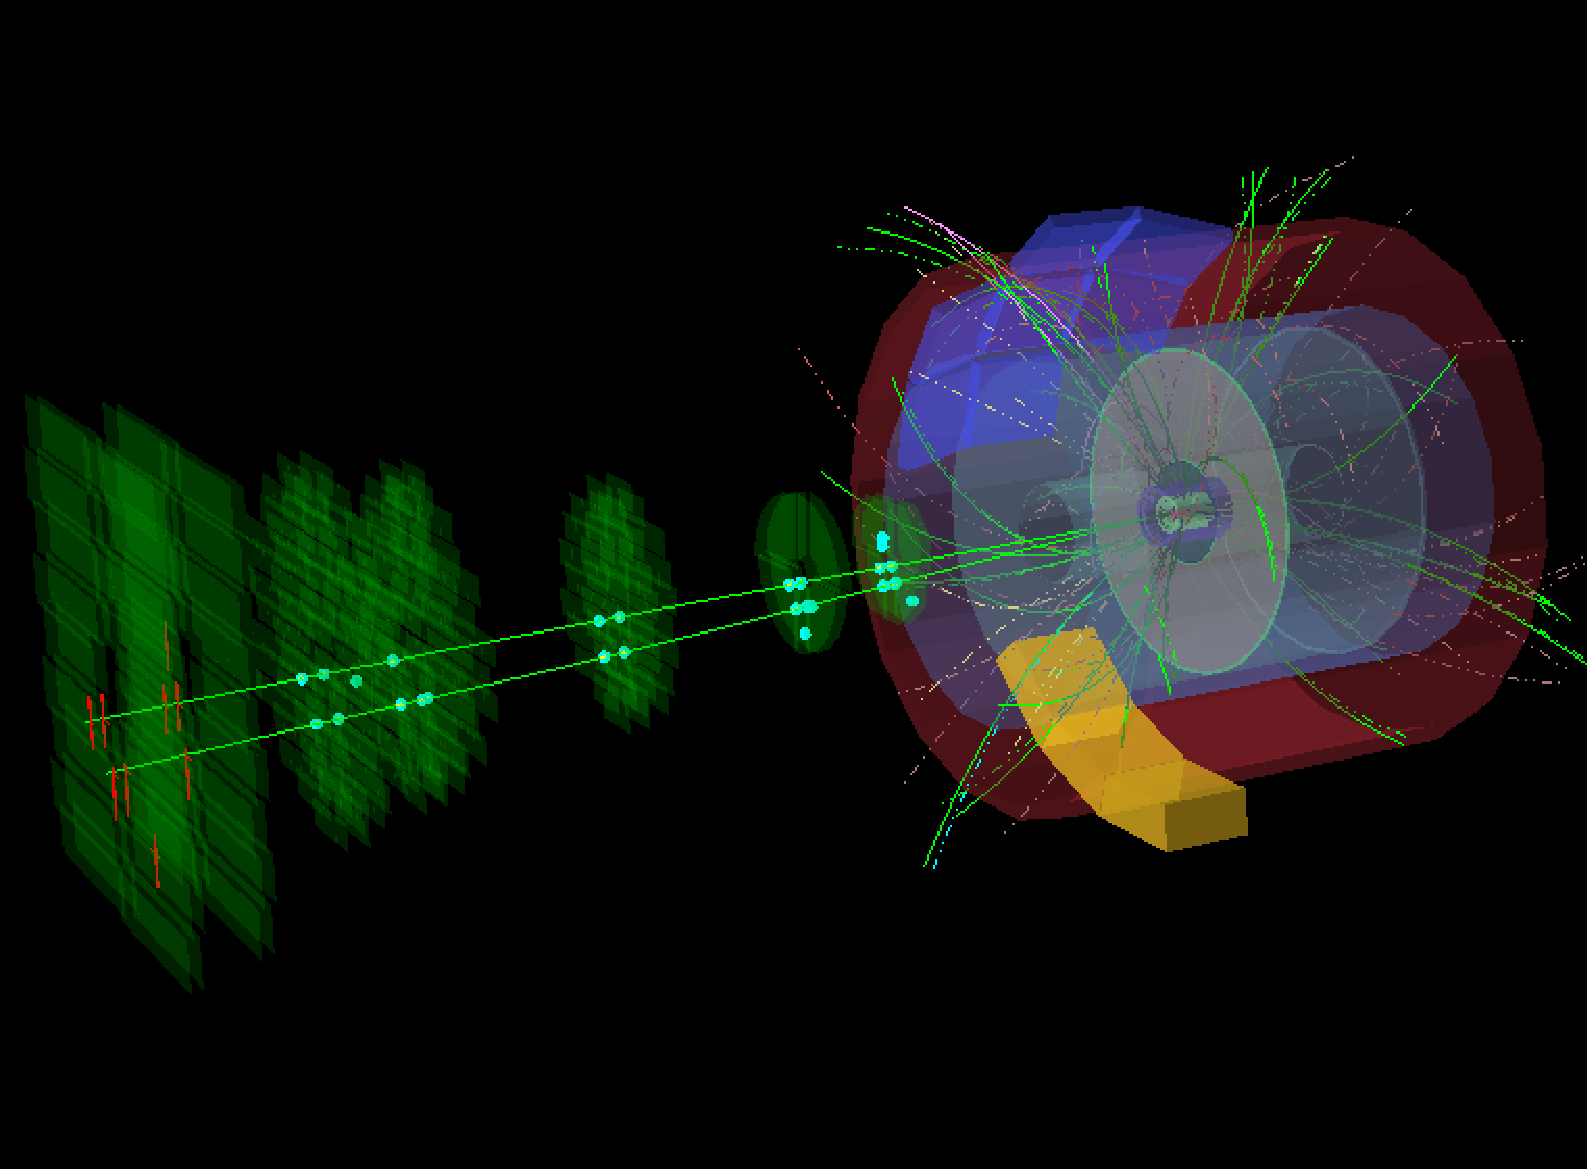
\includegraphics[scale=0.35]{images/7TeVALICEEvent.pdf}
} \\
pp at $\sqrt{s}$=7TeV, 2010 \\
Nucl.Phys. A862-863 (2011) 223-230
\end{frame}

\begin{frame}
  \frametitle{Nominal PbPb event}
\centering{
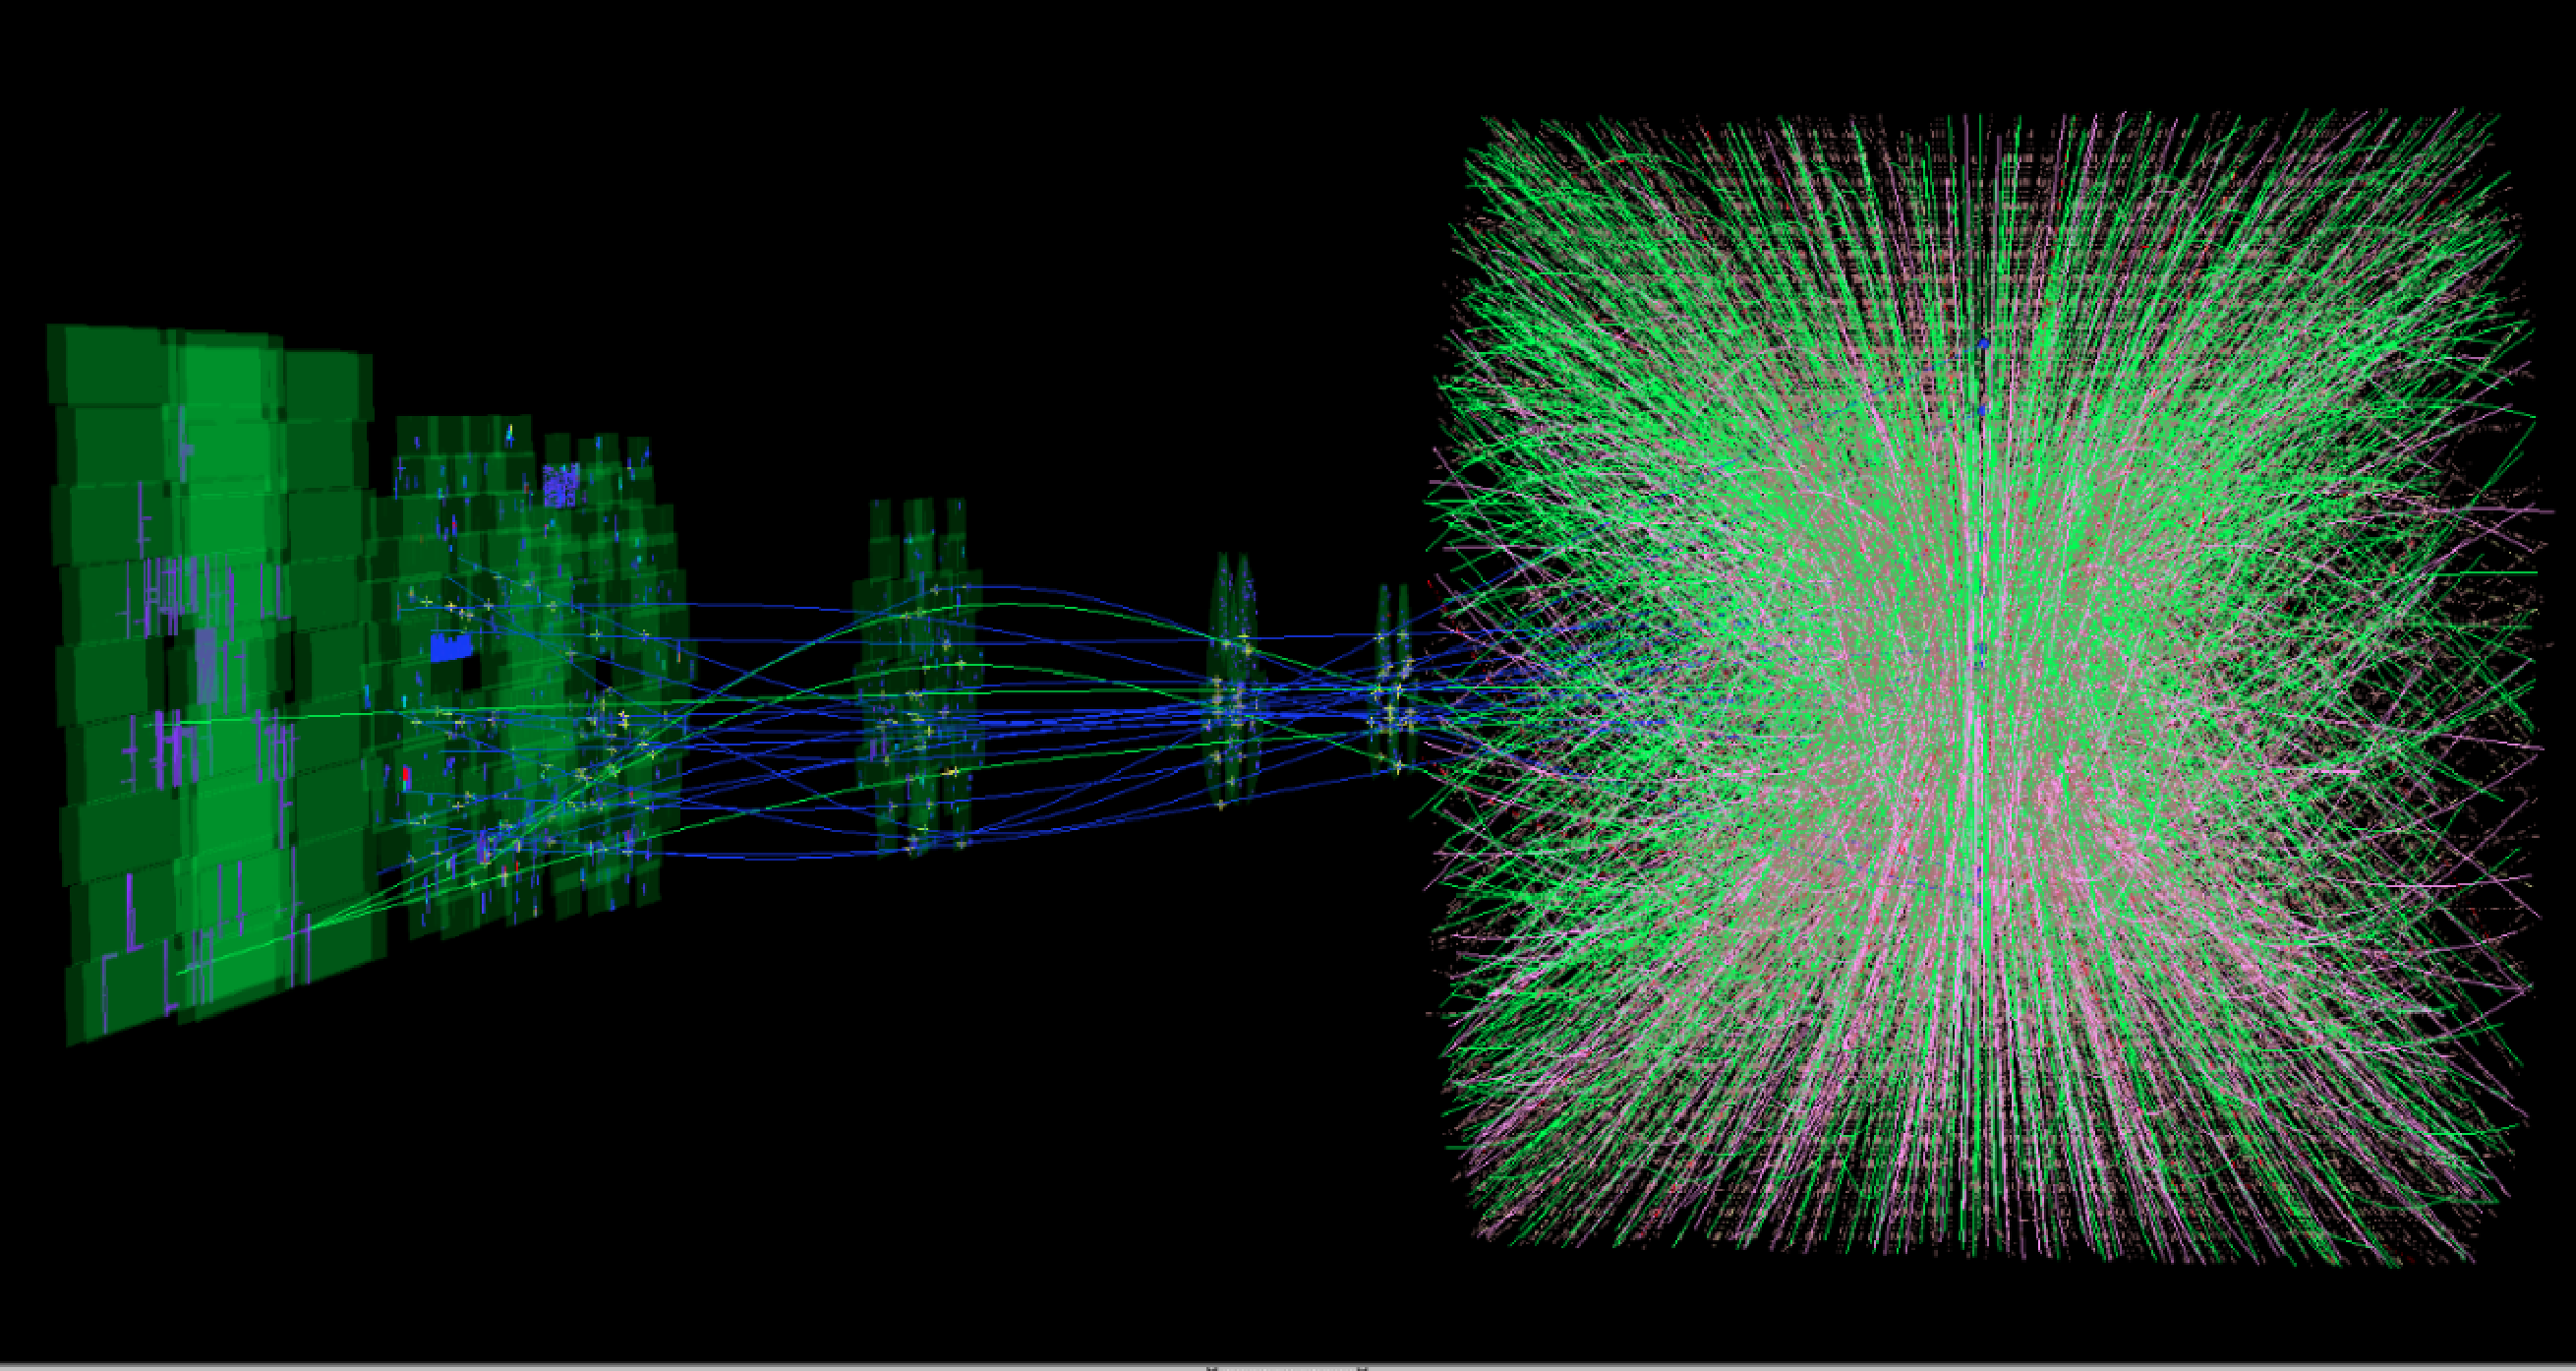
\includegraphics[scale=0.25]{images/HeavyIon.pdf}
} \\
PbPb at $\sqrt{s}$=7 TeV, 2015 \\
\end{frame}

\begin{frame}
  \frametitle{Diagram of detection}

\begin{columns}[T] % align columns
\begin{column}{.48\textwidth}
\begin{itemize}
  \item 100m$^2$ total area
  \item 1.4 million channels
  \item Wire diameter = 20$\mu m$
  \item Wire Pitch : 2$mm$ St1\\
    2.5$mm$ St 2,3,4,5
  \item Pad sizes \\
    \begin{enumerate}
      \item 5x7.5$mm$
      \item 5x15$mm$
      \item 5x30$mm$
    \end{enumerate}
\end{itemize}

\end{column}%
\hfill%
\begin{column}{.48\textwidth}
  \centering{
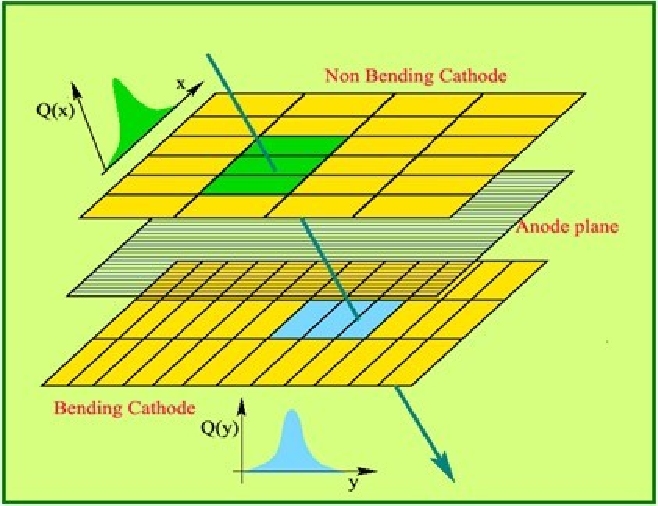
\includegraphics[scale=0.5, angle=90]{images/bendingnonbending.pdf}
} 

\end{column}%
\end{columns}  
  
  
  
\end{frame}


\section{Current MUON Software}

\begin{frame}
\frametitle{Current MUON reconstruction Software}
\begin{itemize}
  \item Raw Data Decoding
  \item Raw Data Filtering
  \item Pre Clustering 
  \item Clusterise, locate cluster interaction point.
  \item Tracking (MCH)
  \item Tracking (MID)
  \item Track Matching MCH-MID
\end{itemize}
\end{frame}
\begin{frame}
  \frametitle{MUON software upgrade in lieu of Run3}
  \begin{itemize}
    \item O(500) times faster at least
    \item Of all computing muon are 15\% of the time spent.
    \item 1.1-1.5s to reconstruct depending on beam.
    \item Aim to have everything online, AOD's out.
    \item Test in current HLT.
  \end{itemize}
\end{frame}
\begin{frame}
  \frametitle{where to start}
  \begin{quote}
\small{There is no doubt that the grail of efficiency leads to abuse. Programmers waste enormous amounts of time thinking about, or worrying about, the speed of non-critical parts of their programs, and these attempts at efficiency actually have a strong negative impact when debugging and maintenance are considered. We should forget about small efficiencies, say about 97\% of the time: premature optimization is the root of all evil.
Yet we should not pass up our opportunities in that critical 3\%. A good programmer will not be lulled into complacency by such reasoning, he will be wise to look carefully at the critical code; but only after that code has been identified.}  
  \end{quote}
Donald Knuth, ACM Computing Surveys, Vol 6, No. 4, Dec. 1974 (see p.268)
\end{frame}

\begin{frame}
  \frametitle{Time Spent}

\begin{tabular}{|l|r|r|r|}
  Function & \multicolumn{3}{c}{Time in \%} \\  
  & pp 16  & PbPb 11 & PbPb 15\\ \hline 
% uncover makes advanced overlay
Raw Data Decoding & 4 & 3&1\\
Raw Data Filtering & 2 & 2&1\\
Pre Clustering & 10 & 10&10\\
Clustering & 63 & 68& 72\\
Tracking MCH & 7 & 6&5 \\
Tracking MID & 6 & 6&6 \\
Track matching & 8 &5 &5 \\
\end{tabular}\\
\vspace{2cm}
\end{frame}

\section{Cluster Finder}

\begin{frame}
\frametitle{What is a cluster finder} 
  \center{
  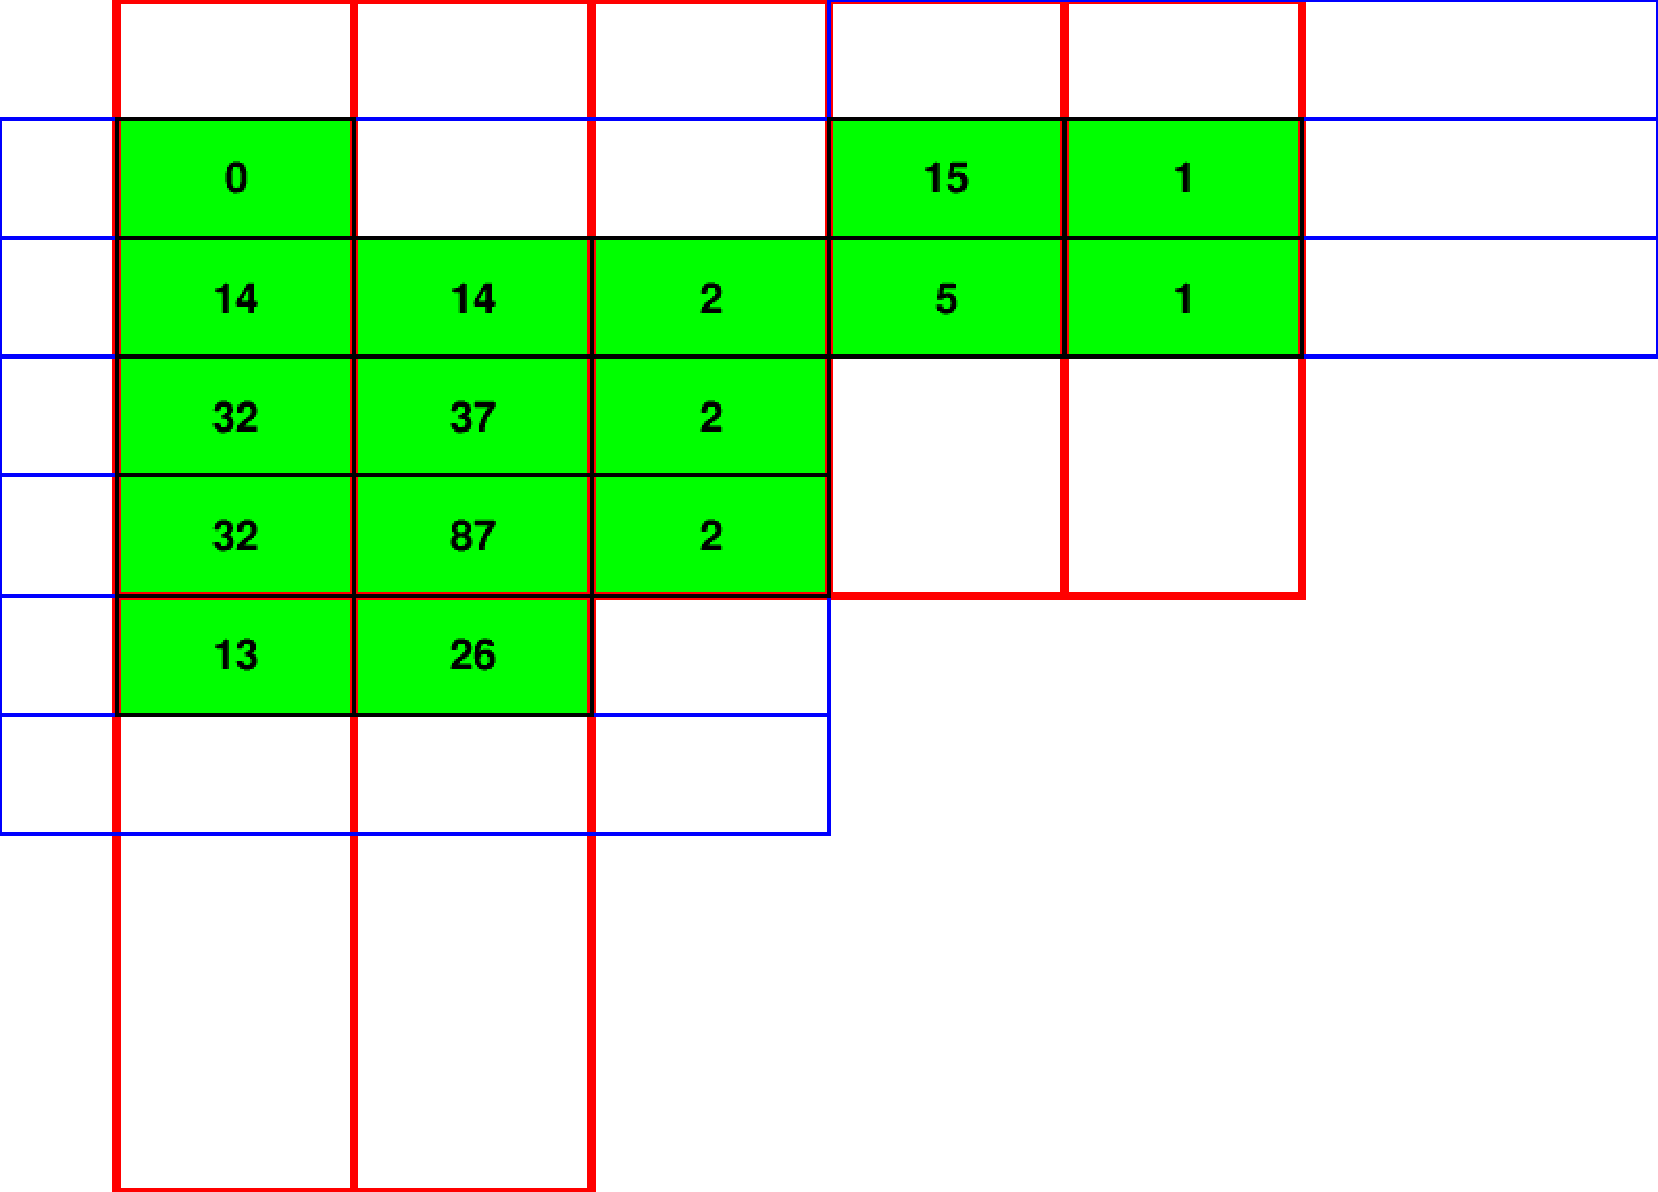
\includegraphics[scale=0.15]{images/mlem_start_EVT26_DE507_CLU-1.pdf}
  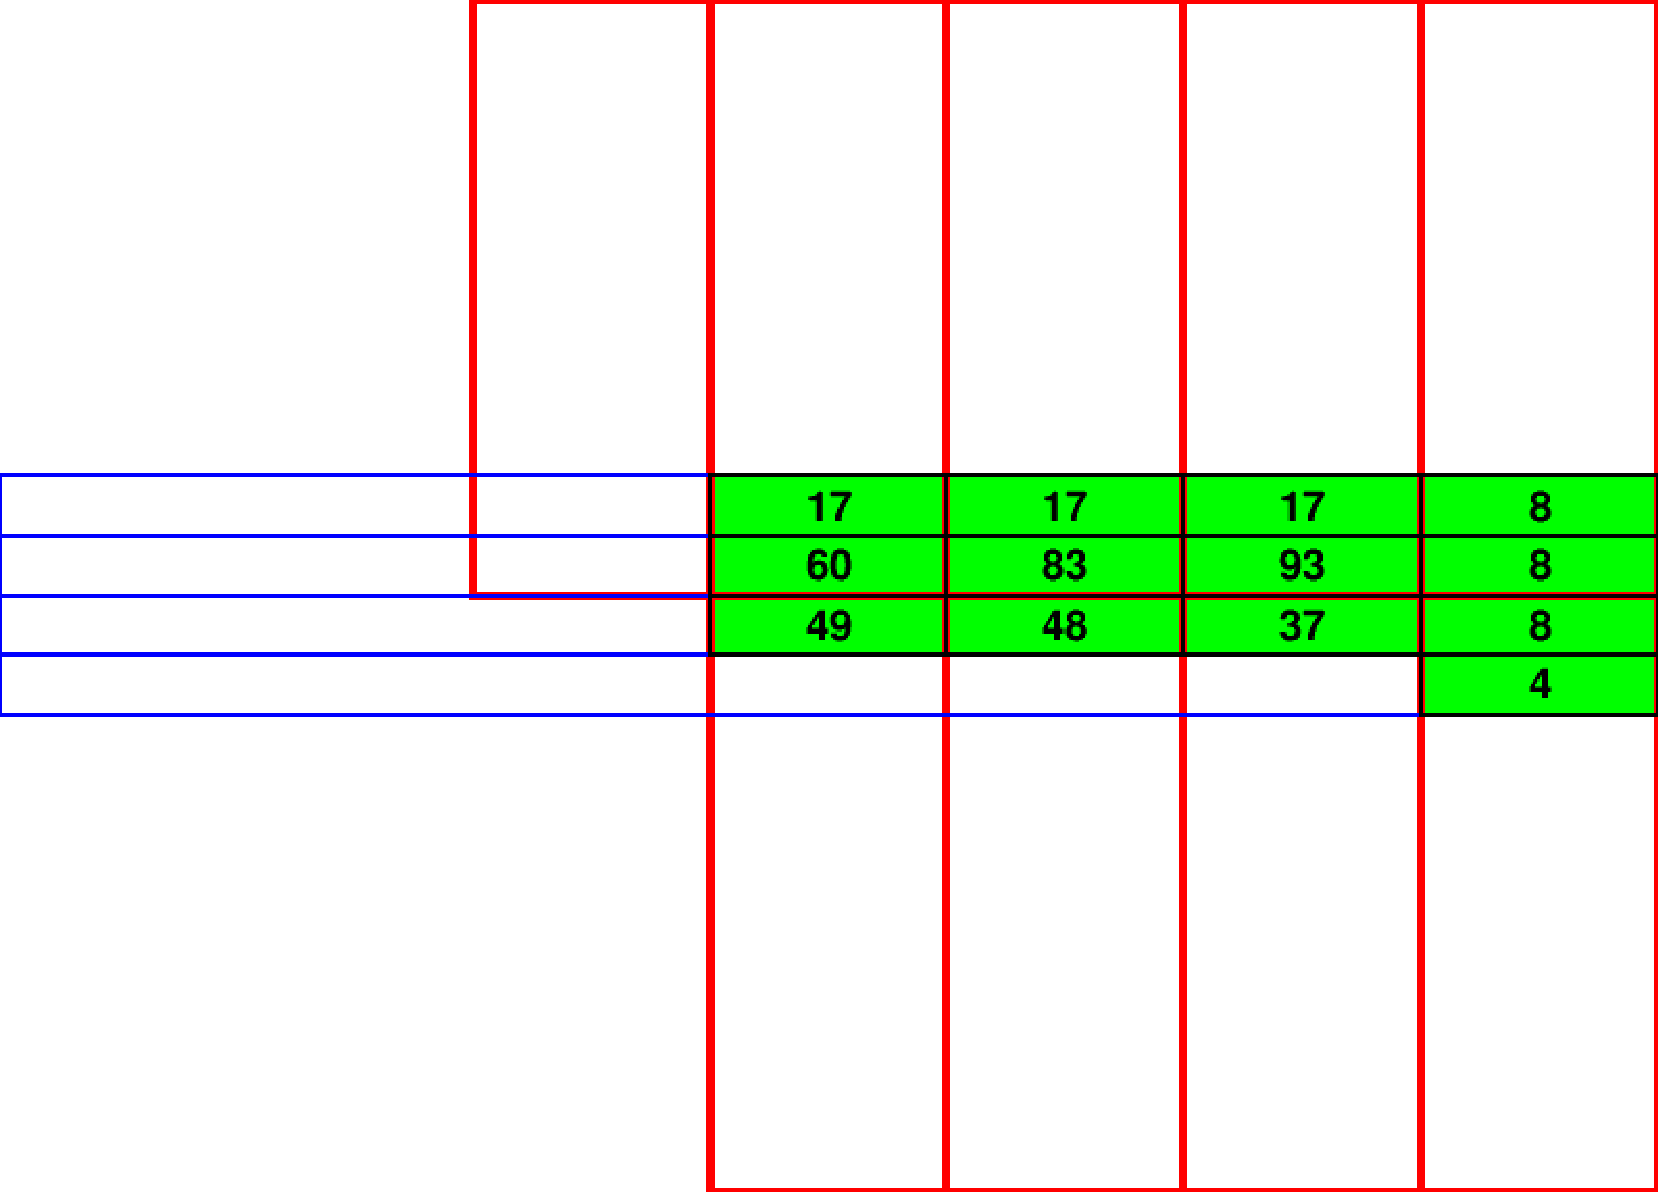
\includegraphics[scale=0.15]{images/mlem_start_EVT26_DE617_CLU-1.pdf}
  }
  % mlem_start_EVT21_DE912_CLU-1.pdf  mlem_start_EVT26_DE507_CLU-1.pdf  mlem_start_EVT26_DE617_CLU-1.pdf  mlem_start_EVT26_DE801_CLU-1.pdf
\end{frame}
\begin{frame}
\frametitle{What is a cluster finder} 
  \center{
  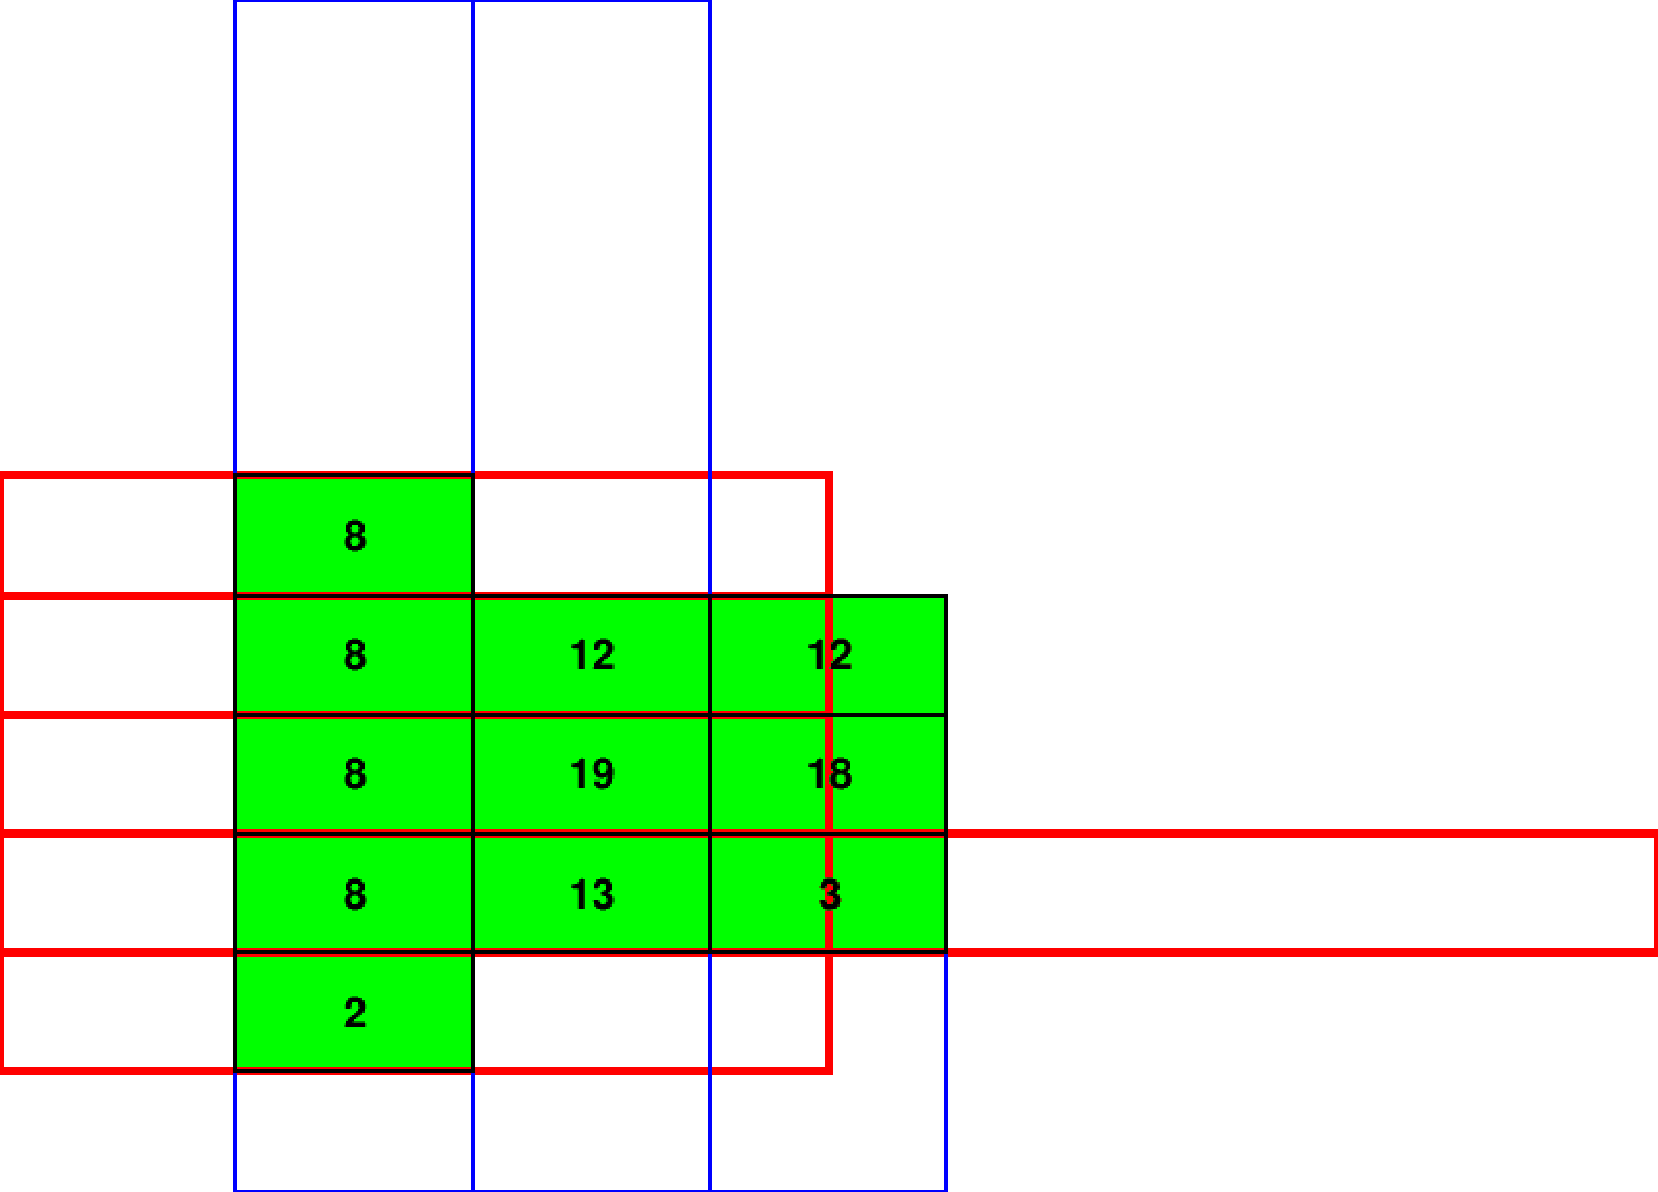
\includegraphics[scale=0.15]{images/mlem_start_EVT26_DE801_CLU-1.pdf}
  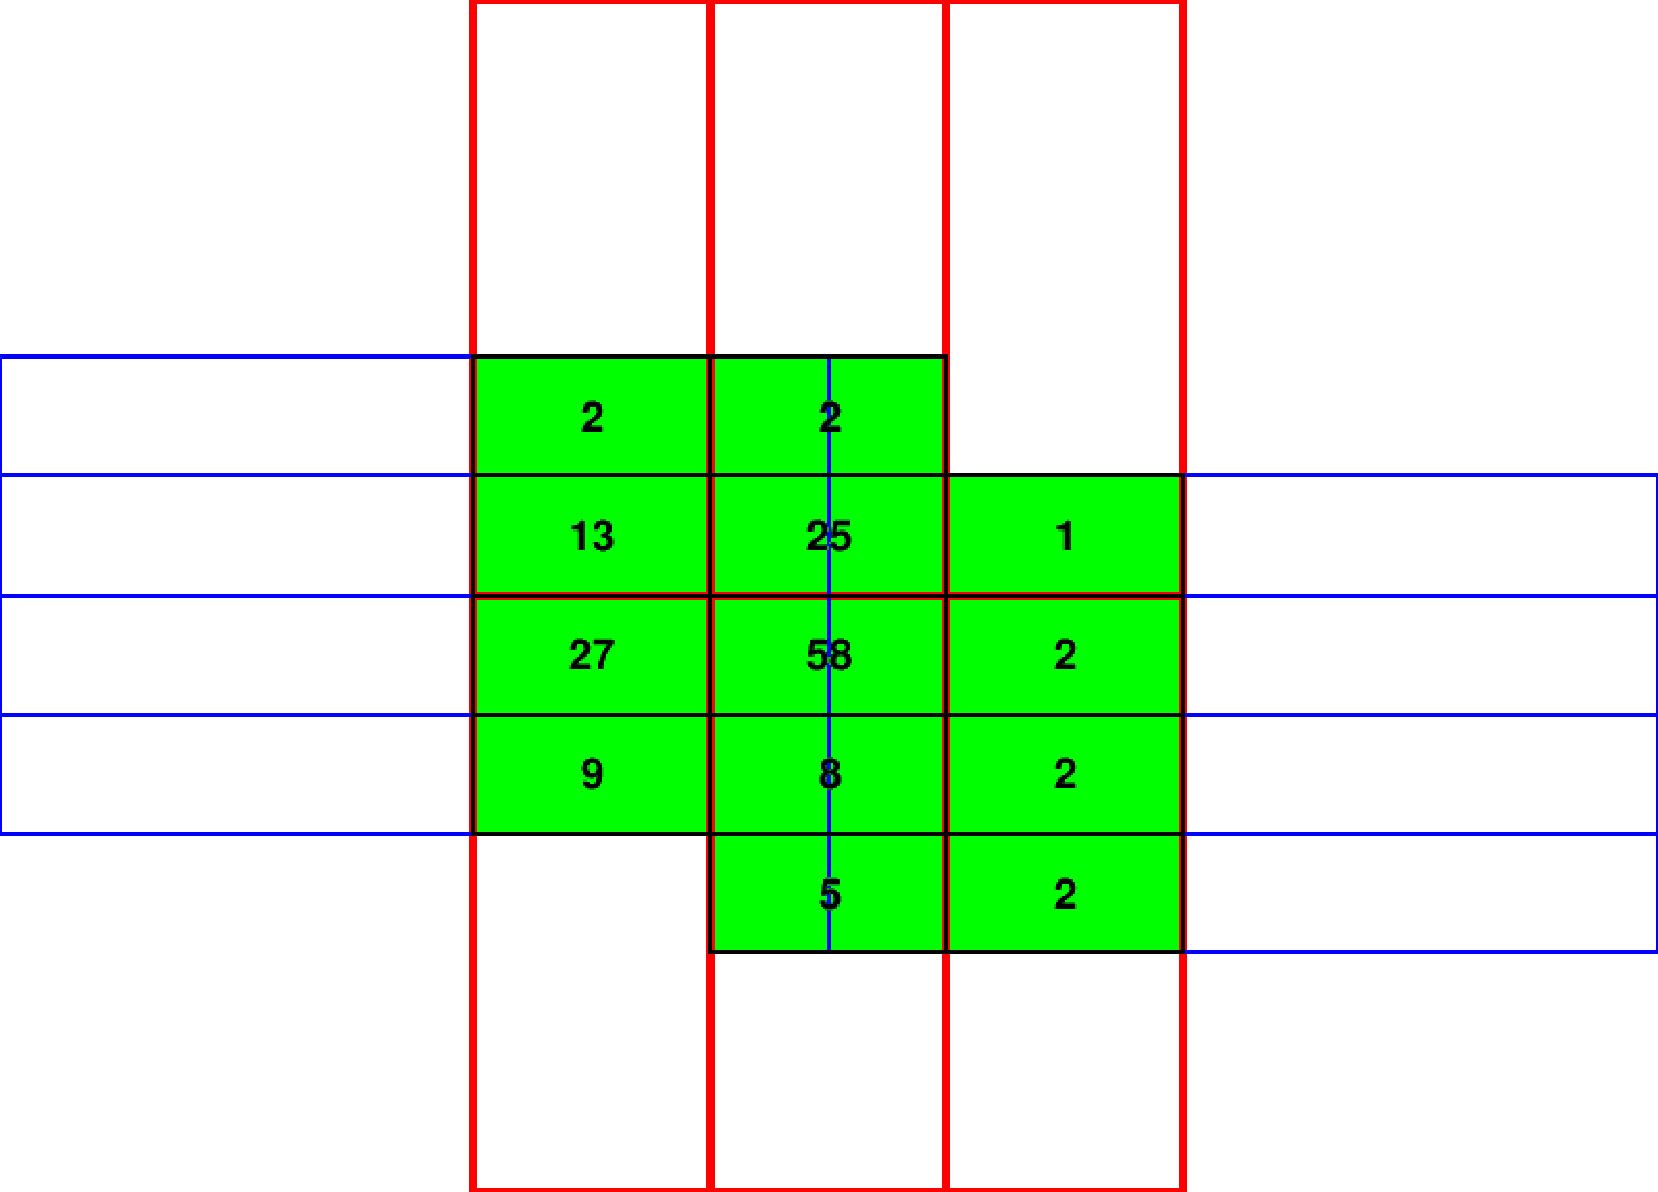
\includegraphics[scale=0.15]{images/mlem_start_EVT21_DE912_CLU-1.pdf} 
  }
  % mlem_start_EVT21_DE912_CLU-1.pdf  mlem_start_EVT26_DE507_CLU-1.pdf  mlem_start_EVT26_DE617_CLU-1.pdf  mlem_start_EVT26_DE801_CLU-1.pdf
\end{frame}

\begin{frame}
  \frametitle{Cluster Mean Size per Chamber PbPb}
  \center{
  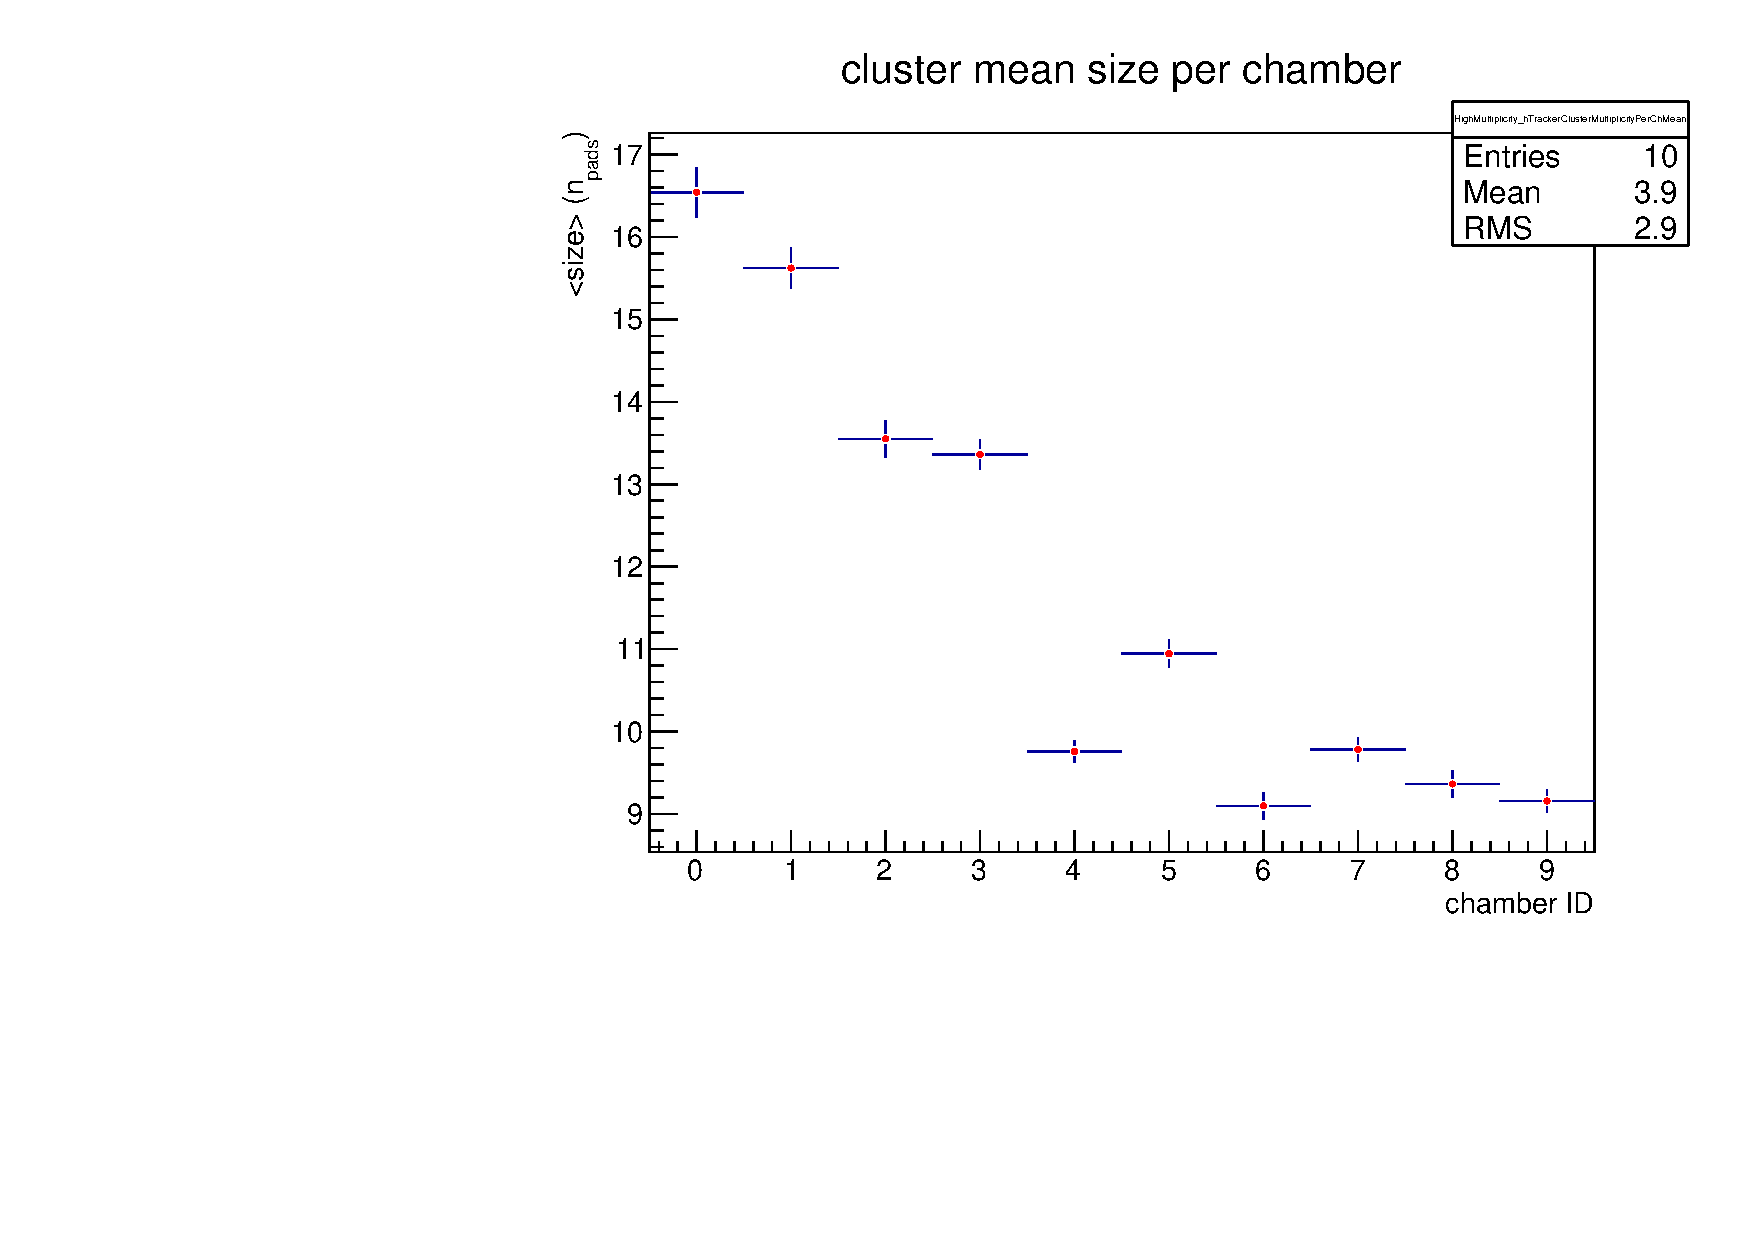
\includegraphics[scale=0.25]{images/ClusterMeanSizerPerChamber_pbpb2015.pdf}
  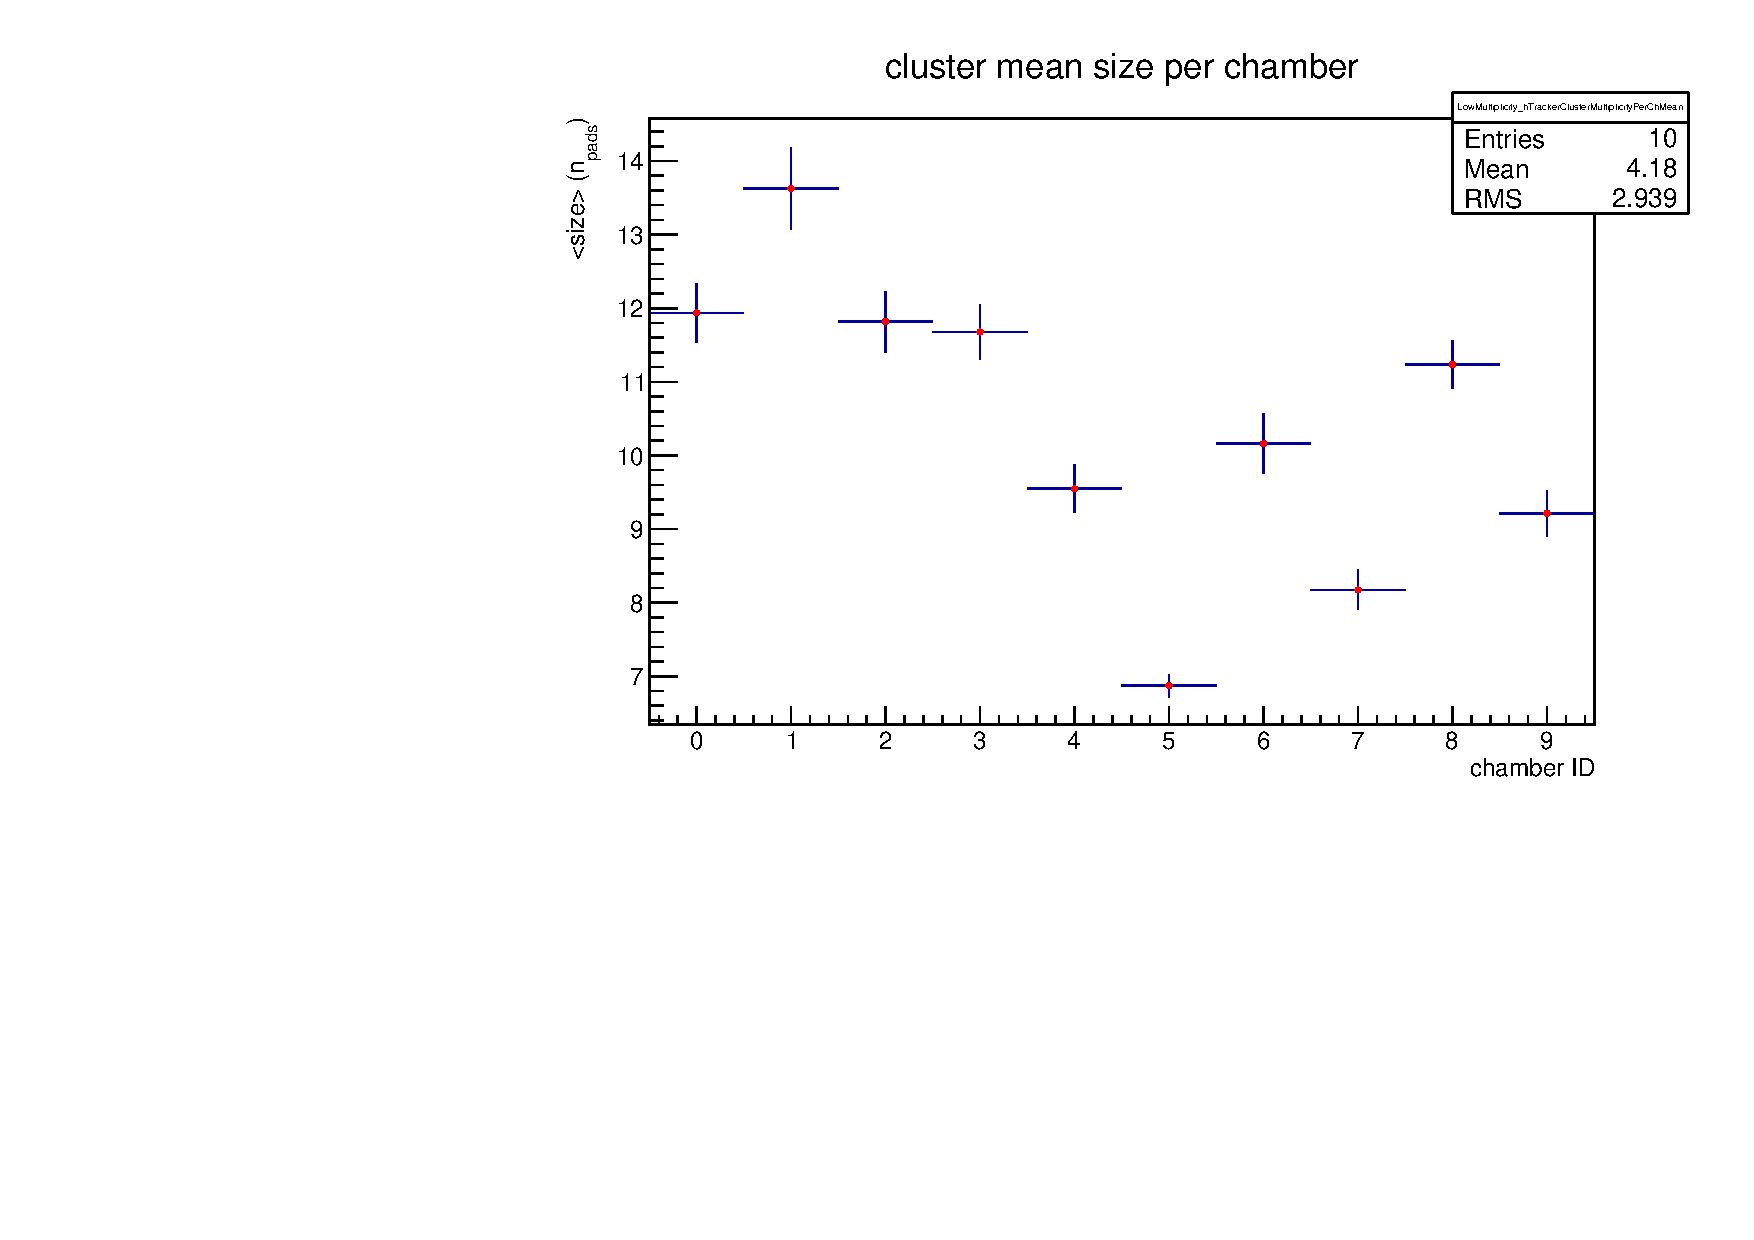
\includegraphics[scale=0.3]{images/ClusterMeanSizerPerChamber_pp2016.pdf}
  }
PbPb 2015 on the left, pp 2016 on the right.
\end{frame}
\begin{frame}
  \frametitle{Cluster Mean Charger per Chamber}
  \center{
  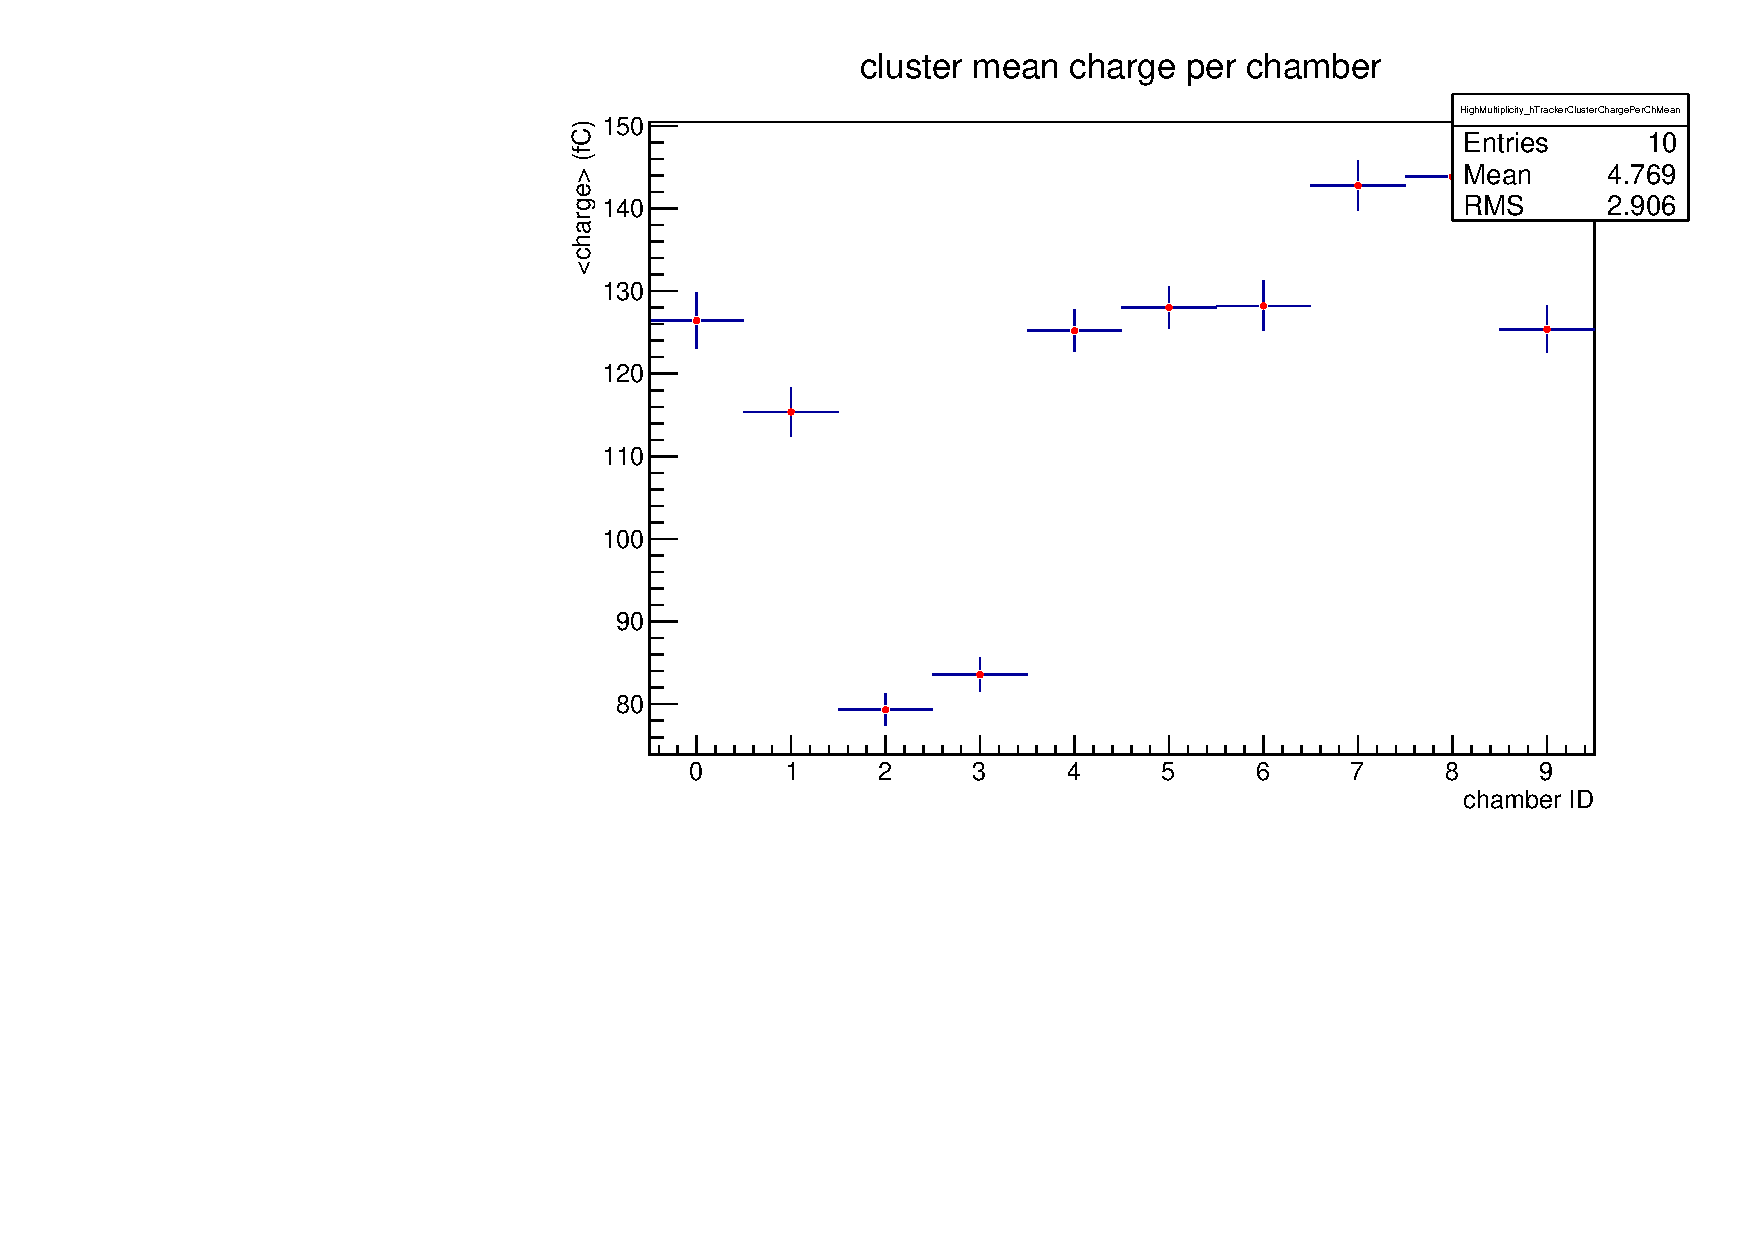
\includegraphics[scale=0.25]{images/ClusterMeanChargePerChamber_pbpb2015.pdf}
  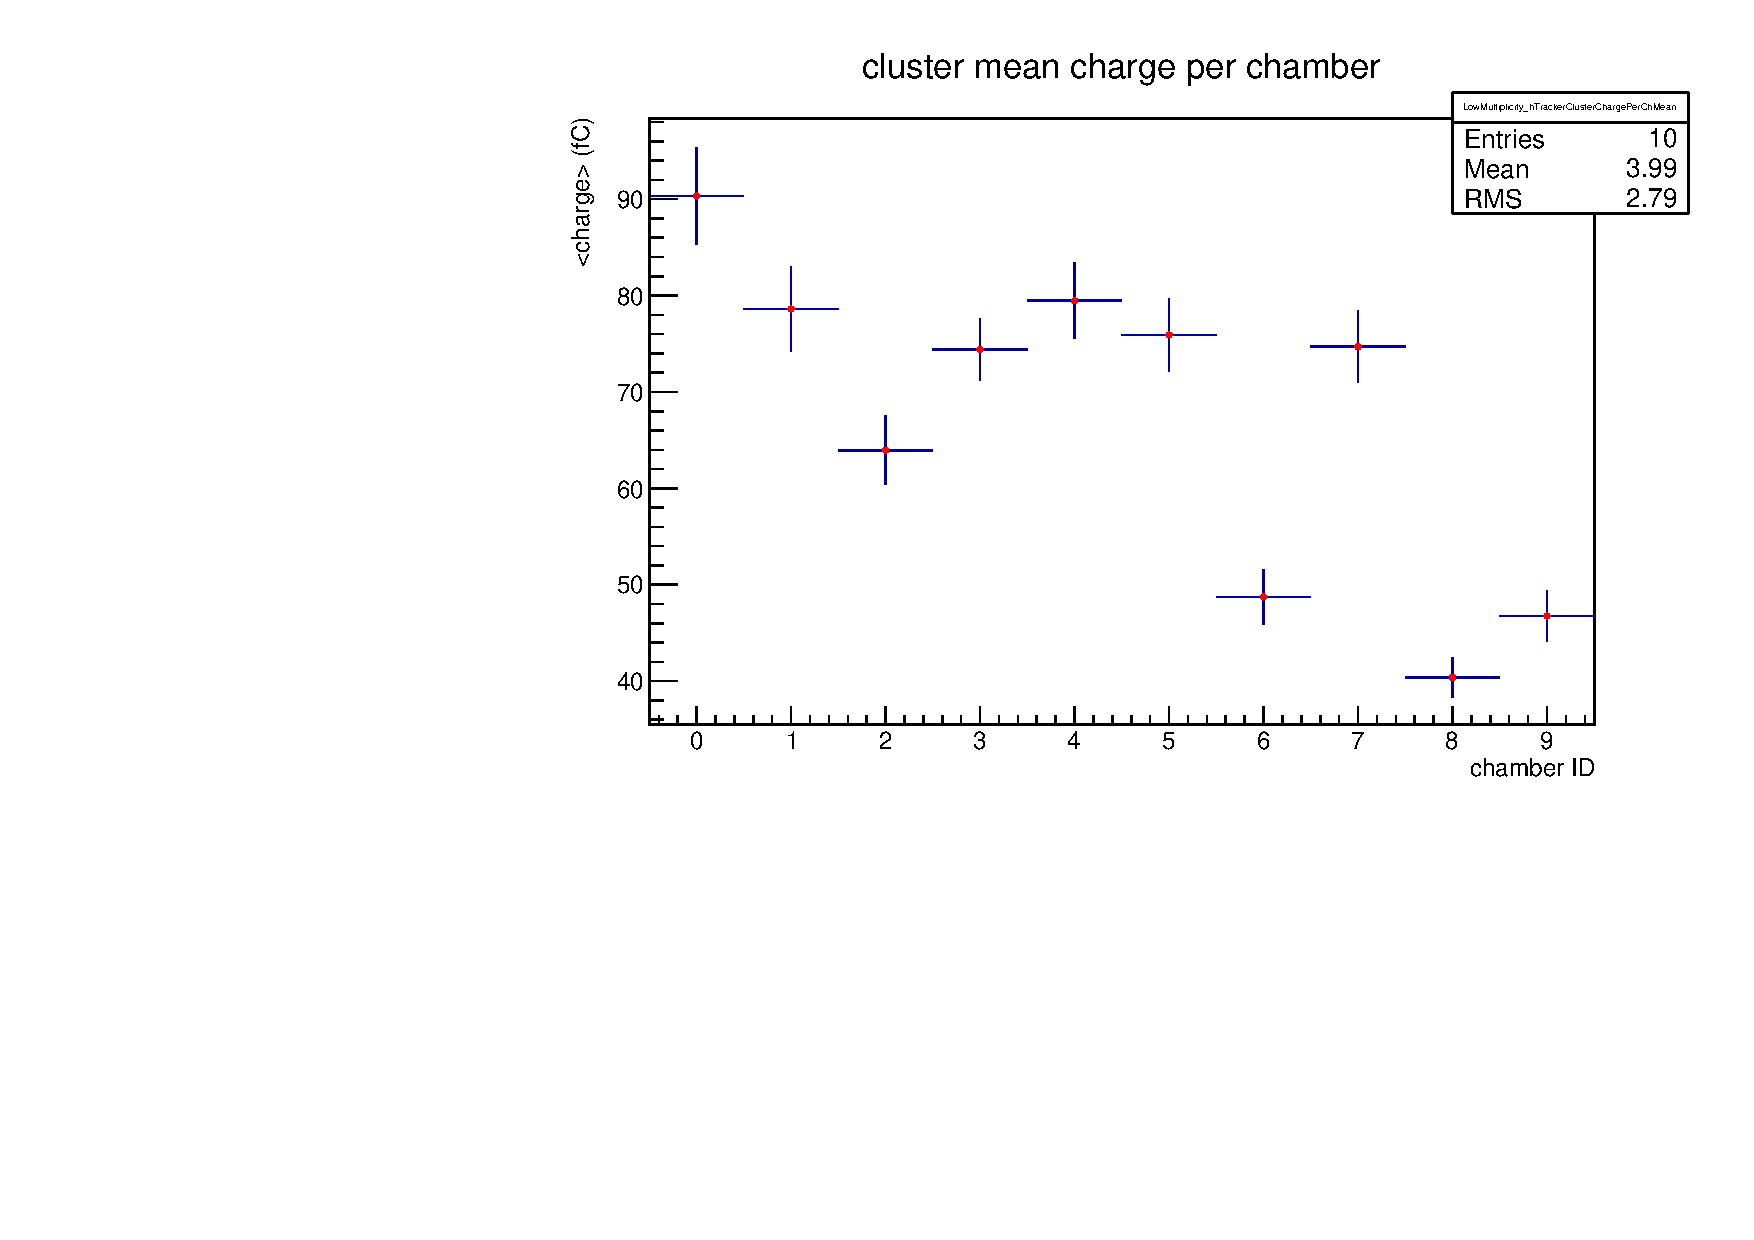
\includegraphics[scale=0.25]{images/ClusterMeanChargePerChamber-pp2016.pdf}
  }

PbPb 2015 on the left, pp 2016 on the right.
\end{frame}

\begin{frame}
  \frametitle{Maximum Likelihood - expectation maximization (MLEM) Algorithm} 
  Used extensively in medical imaging, particularly PET scanners.
  \center{
  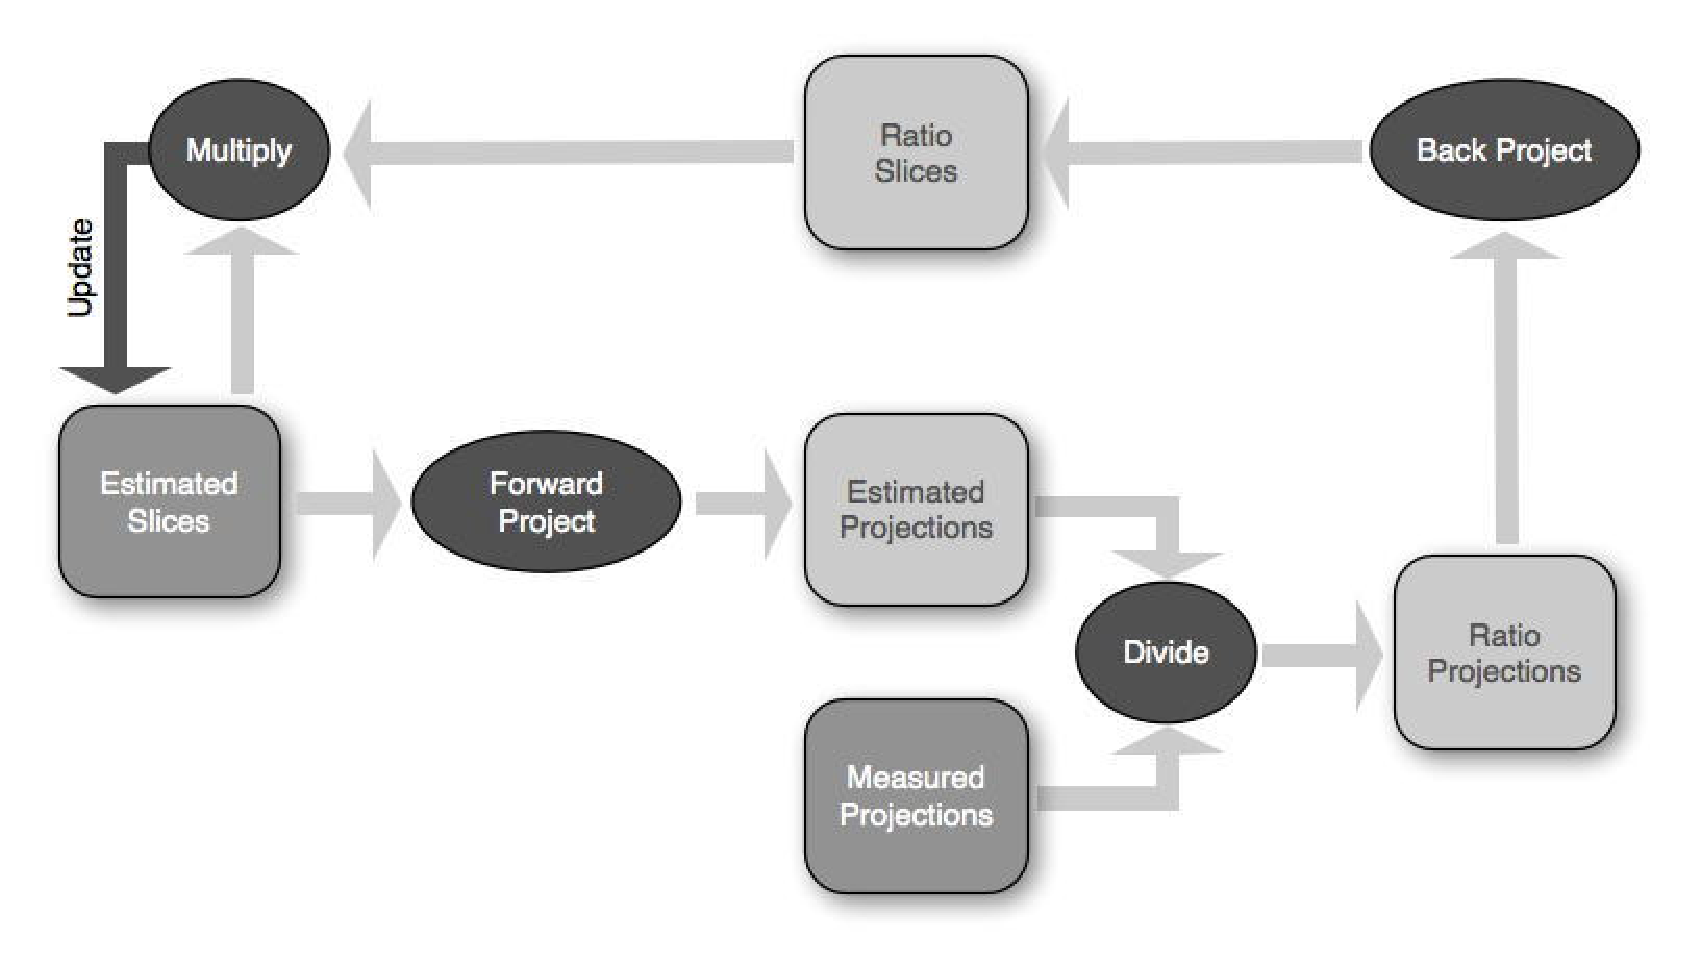
\includegraphics[scale=0.25]{images/MlemIterRecon.pdf}
  }
\end{frame}

\begin{frame}
  \frametitle{MLEM }
  \begin{equation}
    \lambda^{k+1}_j = \frac{\lambda_j^k}{\sum_i^m C_{ij}}\sum^m_i\frac{C_{ij}}{\sum^m_jC_{ij}\lambda_j^k}
  \end{equation}
  \begin{itemize}
    \item $\lambda_j^k$ value of reconstructed charge at $j$ for $k^{th}$ iteration
    \item $y_i$ measured projection data at $i$-th bin
    \item $C_{ij}$ detection probability pixel $j$ to projection bin $i$. The overlapping area pads and pixels in our case.
  \end{itemize}
\end{frame}


\begin{frame}
  \frametitle{Logical Parts}
  \begin{enumerate}
    \item Add Virtual pads if necessary, smooth out holes.
    \item MLEM until sufficiently small pixel size is achieved.
    \item Find Center of Gravity around maximal pixel
    \item loop back with smaller and smaller pixels
    \item Remove Pixels with low signal or visibility, preserving charge to nearest neighbor.
    \item MLEM algorithm again.
  \end{enumerate}
  MLEM :
  \begin{itemize}
      \item 4 way nested dependent loops.
  \end{itemize}
\end{frame}


\begin{frame}
  \frametitle{Speed up}
\begin{itemize}
  \item look for dead code 11\% (Finding nearest neighbor)
  \item change data or reorder to hit caches better. 5\%
  \item get a faster cpu. sadly not going to happen 
  \item gpu 30\%, but 4 nested dependent loops
  \item fpga - try to avoid.
  \item do something completely different.
\end{itemize}
Performed on a i7 with nvidia gtx 980, will have to be repeated on other hardware.
\end{frame}

\begin{frame}
\frametitle{Something else}
At this stage now.
\end{frame}

\end{document}

